%% For double-blind review submission, w/o CCS and ACM Reference (max submission space)
%\documentclass[acmsmall,review]{acmart}\settopmatter{printfolios=true,printccs=false,printacmref=false}
%% For double-blind review submission, w/ CCS and ACM Reference
\documentclass[acmsmall,review,anonymous,screen]{acmart}\settopmatter{printfolios=true,printacmref=false}
%% For double-blind review submission, w/ CCS and ACM Reference
%\documentclass[acmsmall,screen]{acmart}\settopmatter{printfolios=true,printacmref=false}
%% For single-blind review submission, w/o CCS and ACM Reference (max submission space)
%\documentclass[acmsmall,review]{acmart}\settopmatter{printfolios=true,printccs=false,printacmref=false}
%% For single-blind review submission, w/ CCS and ACM Reference
%\documentclass[acmsmall,review]{acmart}\settopmatter{printfolios=true}
%% For final camera-ready submission, w/ required CCS and ACM Reference
%\documentclass[acmsmall]{acmart}\settopmatter{}
\usepackage[shortlabels]{enumitem}
\usepackage{mathtools}
\usepackage{wrapfig}
\usepackage{stackengine}
\usepackage{ textcomp }

\DeclareSymbolFont{arrows}{U}{FdSymbolC}{m}{n}

% \usepackage{ amssymb }
\DeclareTextFontCommand{\texttt}{\ttfamily}

%% Journal information
%% Supplied to authors by publisher for camera-ready submission;
%% use defaults for review submission.
\acmJournal{PACMPL}
\acmVolume{}
\acmNumber{OOPSLA} % CONF = POPL or ICFP or OOPSLA
\acmArticle{}
\acmYear{2025}
\acmMonth{1}
\acmDOI{} % \acmDOI{10.1145/nnnnnnn.nnnnnnn}
\startPage{1}

%% Copyright information
%% Supplied to authors (based on authors' rights management selection;
%% see authors.acm.org) by publisher for camera-ready submission;
%% use 'none' for review submission.
\setcopyright{none}
%\setcopyright{acmcopyright}
%\setcopyright{acmlicensed}
%\setcopyright{rightsretained}
%\copyrightyear{2018}           %% If different from \acmYear

%% Bibliography style
\bibliographystyle{ACM-Reference-Format}
%% Citation style
%% Note: author/year citations are required for papers published as an
%% issue of PACMPL.
%\citestyle{acmauthoryear}   %% For author/year citations
\citestyle{acmnumeric}

%%%%%%%%%%%%%%%%%%%%%%%%%%%%%%%%%%%%%%%%%%%%%%%%%%%%%%%%%%%%%%%%%%%%%%
%% Note: Authors migrating a paper from PACMPL format to traditional
%% SIGPLAN proceedings format must update the '\documentclass' and
%% topmatter commands above; see 'acmart-sigplanproc-template.tex'.
%%%%%%%%%%%%%%%%%%%%%%%%%%%%%%%%%%%%%%%%%%%%%%%%%%%%%%%%%%%%%%%%%%%%%%


%% Some recommended packages.
\usepackage{booktabs}   %% For formal tables:
                        %% http://ctan.org/pkg/booktabs
\usepackage{subcaption} %% For complex figures with subfigures/subcaptions
                        %% http://ctan.org/pkg/subcaption
 \usepackage{ stmaryrd }                       

\usepackage{relsize}
\usepackage{mathpartir}
\usepackage{amsmath}
\usepackage{amsthm}
\usepackage{listings}
\usepackage{xspace}
\usepackage{definitions}
\usepackage{multirow,bigdelim}
\usepackage{pbox}
\usepackage{courier}
\usepackage{soul}
\usepackage{centernot}
\usepackage{dutchcal}
%\usepackage{pzccal} 
%\DeclareFontFamily{OT1}{pzc}{}
%\DeclareFontShape{OT1}{pzc}{m}{it}{<-> s * [1.10] pzcmi7t}{}
%\DeclareMathAlphabet{\mathpzc}{OT1}{pzc}{m}{it}

\newcommand\multibrace[3]{\rdelim\}{#1}{3mm}[\pbox{#2}{#3}]}


%%these COLOUR MACROS ARE ACTIVELY FUCKING EVIL
%%DO NOT DO THIS. EVER
%%AT LEast have some ovious way to TURN THEM OFF

\definecolor{ferngreen}{rgb}{0.31, 0.47, 0.26}
\newcommand{\kjx}[1]{{}}
\newcommand{\scd}[1]{{}}
%\newcommand{\sdN}[1]{{\color{dkgreen}{#1}}}
%\newcommand{\jm}[1]{{\color{magenta}{JM: #1}}}
\newcommand{\sdcomment}[1]{{}}
\newcommand{\secomment}[1]{{}}
\newcommand{\jncomment}[1]{{}}

\newcommand{\sd}[1]{{{#1}}}
\newcommand{\se}[1] {#1} %{{\color{brown}{#1}}}
\newcommand{\sue}[1] {{\color{brown}{#1}}}
\definecolor{amber}{rgb}{1.0, 0.75, 0.0}
\definecolor{amethyst}{rgb}{0.6, 0.4, 0.8}

\newcommand{\ponders}[3]{\marginpar{\tiny\itshape\raggedright\textcolor{#2}{\textbf{#1:} #3}}\ignorespaces}
\renewcommand{\ponders}[3]{{#3\ignorespaces}}  %TURNING IT OFF. NOT THAT IT FUCKING HEPLS

\marginparwidth=1.6cm \marginparsep=0cm
\newcommand{\TODO}[1]{} % {{\color{red}#1}}
\newcommand{\sophia}[1]{{#1}}
\newcommand{\toby}[1]{} % {\ponders{Toby}{purple}{#1}}
\newcommand{\susan}[2][]{{#2}\xspace}
\newcommand{\james}[1]{\ponders{James}{orange}{#1}}
\newcommand{\jm}[2][]{\ponders{Julian}{magenta}{#1} {#2}\xspace}
\newcommand{\mrr}[2][]{\ponders{Matthew Ross}{offblue}{{#1}} {{#2}}\xspace}
\newcommand{\sdNr}[2][]{\ponders{SD:}{amber}{#1} {#2}\xspace}
\newcommand{\sdN}[1]{{{#1}}}
\newcommand{\sdNO}[1]{\red{ {#1}}} %{\ponders{SD:}{amber}{ } {#1}\xspace}
\newcommand{\julian}[1]{{#1}\xspace}
\newcommand{\sdM}[1]{#1\xspace}

\newcommand{\sophiaPonder}[2][]{\ponders{Sophia}{blue}{#1}{#2}\xspace}
\renewcommand{\sophia}[2][]{}

\newcommand{\sdfootnote}[1]{}



\begin{document}

%% Title information
%\title[Specification and Proof of Necessary Conditions]{Specification
%and Proof of Necessary Conditions}         %% [Short Title] is
%optional;
%\title{Necessity Specifications are Necessary
%\title{Reasoning about External Calls with Limited Effects}
\title{Reasoning about Trust and Risk -- revisited}
%\title{Limiting the Effects of External Calls}
%\title{Limited Effects for Reasoning about External Calls}
%\title{Reasoning about External Calls}

% \title{\Nec Specifications are Necessary for Robustness}

                                        %% when present, will be used in
                                        %% header instead of Full Title.
%\titlenote{with title note}             %% \titlenote is optional;
                                        %% can be repeated if necessary;
                                        %% contents suppressed with 'anonymous'
%\subtitle{Subtitle}                     %% \subtitle is optional
%\subtitlenote{with subtitle note}       %% \subtitlenote is optional;
                                        %% can be repeated if necessary;
                                        %% contents suppressed with 'anonymous'


%% Author information
%% Contents and number of authors suppressed with 'anonymous'.
%% Each author should be introduced by \author, followed by
%% \authornote (optional), \orcid (optional), \affiliation, and
%% \email.
%% An author may have multiple affiliations and/or emails; repeat the
%% appropriate command.
%% Many elements are not rendered, but should be provided for metadata
%% extraction tools.
 



%% Author with two affiliations and emails.
\author{Julian Mackay}
%\authornote{with author2 note}          %% \authornote is optional;
                                        %% can be repeated if necessary
\orcid{0000-0003-3098-3901}             %% \orcid is optional
\affiliation{
  %\position{Position2a}
  %\department{Engineering and Computer Science}             %% \department is recommended
  \institution{Victoria University of Wellington}           %% \institution is required
  %\streetaddress{Street2a Address2a}
  %\city{City2a}
  %\state{State2a}
  %\postcode{Post-Code2a}
   \country{NZ}   % \country{New Zealand}                   %% \country is recommended
}
\email{julian.mackay@ecs.vuw.ac.nz}         %% \email is recommended


\author{Susan Eisenbach}
%\authornote{with author2 note}          %% \authornote is optional;
                                        %% can be repeated if necessary
\orcid{0000-0001-9072-6689}             %% \orcid is optional
\affiliation{
  %\position{Position2a}
  %\department{}             %% \department is recommended
  \institution{Imperial College London}           %% \institution is required
  %\streetaddress{Street2a Address2a}
  %\city{City2a}
  %\state{State2a}
  %\postcode{Post-Code2a}
  \country{UK} %   \country{United Kingdom}                   %% \country is recommended
}
\email{susan@imperial.ac.uk}         %% \email is recommended

\author{James Noble}
%\authornote{with author2 note}          %% \authornote is optional;
                                        %% can be repeated if necessary
\orcid{0000-0001-9036-5692}             %% \orcid is optional
\affiliation{
  %\position{Position2a}
  %\department{Department2a}             %% \department is recommended
  \institution{Creative Research \& Programming}           %% \institution is required
 % \streetaddress{5 Fernlea Ave, Darkest Karori}
  \city{Wellington}
  %\state{State2a}
  \postcode{6012}
   \country{NZ}   %  \country{New Zealand}                   %% \country is recommended
}
\email{kjx@acm.org}         %% \email is recommended

%% Author with single affiliation.
\author{Sophia Drossopoulou}
%\authornote{with author1 note}          %% \authornote is optional;
                                        %% can be repeated if necessary
\orcid{0000-0002-1993-1142}             %% \orcid is optional
\affiliation{
  %\position{Position1}
  %\department{Department1}              %% \department is recommended
  \institution{Imperial College London}            %% \institution is required
  %\streetaddress{Street1 Address1}
  %\city{City1}
  %\state{State1}
  %\postcode{Post-Code1}
  \country{UK} %  \country{United Kingdom}                    %% \country is recommended
}
\email{scd@imperial.ac.uk}          %% \email is recommended


%% Abstract
%% Note: \begin{abstract}...\end{abstract} environment must come
%% before \maketitle command


  

%% 2012 ACM Computing Classification System (CSS) concepts
%% Generate at 'http://dl.acm.org/ccs/ccs.cfm'.
\begin{CCSXML}
<ccs2012>
   <concept>
       <concept_id>10011007.10010940.10010992.10010993.10011683</concept_id>
       <concept_desc>Software and its engineering~Access protection</concept_desc>
       <concept_significance>300</concept_significance>
       </concept>
   <concept>
       <concept_id>10011007.10011074.10011099.10011692</concept_id>
       <concept_desc>Software and its engineering~Formal software verification</concept_desc>
       <concept_significance>500</concept_significance>
       </concept>
   <concept>
       <concept_id>10003752.10003790.10011741</concept_id>
       <concept_desc>Theory of computation~Hoare logic</concept_desc>
       <concept_significance>500</concept_significance>
       </concept>
   <concept>
       <concept_id>10011007.10011006.10011008.10011009.10011011</concept_id>
       <concept_desc>Software and its engineering~Object oriented languages</concept_desc>
       <concept_significance>300</concept_significance>
       </concept>
 </ccs2012>
\end{CCSXML}

\ccsdesc[300]{Software and its engineering~Access protection}
\ccsdesc[500]{Software and its engineering~Formal software verification}
\ccsdesc[500]{Theory of computation~Hoare logic}
\ccsdesc[300]{Object oriented programming~Object capabilities}



%% End of generated code

  
%% End of generated code


%% Keywords
%% comma separated list
%%%%%%%%%%%%%%%%%%%%%\keywords{keyword1, keyword2, keyword3}  %% \keywords are mandatory in final camera-ready submission



%% Note: \maketitle command must come after title commands, author
%% commands, abstract environment, Computing Classification System
%% environment and commands, and keywords command.


 %  \begin{abstract}
 
 
 In today's complex software, internal, trusted, code  is tightly intertwined  
 with external, untrusted, code. %: external code
 %may call
% calls
% into internal code, internal code
% may call
% calls
% out to external code,
% and external code
 %  may then call back
%even calls back 
% into internal code.
% In particular, trusted  code may be called by external, unverified,
% untrusted code; moreover, it may call such external, unverified,
% untrusted code
By definition, internal code does not trust external code.
From an internal perspective, the effects of
outgoing calls to external code -- \emph{external calls} ---
are %in principle
necessarily
unknown and unlimited.

Nevertheless, the effects of external calls can be \emph{\tamed}
% , \ie reduced, \
if internal code % module %makes use of encapsulation and
is programmed defensively,
%\ie to prevent some effects from happening.
\ie to ensure particular effects cannot happen.
\Tamed effects allow us to prove that internal code
preserves assertions about internal and external objects,
even in the presence of outgoing calls and callbacks.
%
%  external calls will preserve some {why only some?} assertions.
%
%% {Given that this is the abstract I would skip the next two
%%   sentences.}
%% \kjx{skipped}
%% To \tame effects, one needs to use encapsulation (\eg private fields, no address forging, \etc). 
%% One may also employ  the OCAP (object capabilities) model, whereby 
%% % capabilities are transferable rights to perform one or more operations on a given object;
% access to the capability is  necessary for some  effect to  happen.
%Capabilities are unforgeable, and can only be acquired through explicit passing from caller to callee, or at object creation.
 % As a result, sharing of capabilities has to be carefully managed.
%

This paper
addresses the specification and verification of internal code,
using encapsulation and object capabilities to \tame effects.
We propose new assertions for access to capabilities,
new specifications for \tamed effects,
and a Hoare logic to verify that a module satisfies its \tamed
effects specification, even while making external calls.
We illustrate the approach though a running example,
and prove soundness of the Hoare logic.


 \forget{
%Our work
This paper
addresses the specification and verification of internal code
which uses encapsulation and object capabilities to \tame effects.
%{Are they assertions and specifications or assertion constructs
%and specification language?}
%kjx: shorter is better
We propose new assertions talking about access to capabilities,
new specifications describing \tamed effects,
%kjx howmany Hoare logics??
%a Hoare logic that can verify external calls,
and a Hoare logic that can verify that a module satisfies its \tamed
effects specification, even while making external calls.
We illustrate the approach though a running example,
and prove soundness of the Hoare logic.
%% -- something not yet sufficiently  tackled by the OCAP  literature.
%{\textbf {For the specification:}} To%  not being ``entitled'' to some effect, we give a means to guarantee  that lack of (eventual) access to certain capabilities ensures
%that certain effects will not take place.
% To reflect that the guarantees
%should hold in the presence of internal code calling and being called by external code, we 
%% are about eventual} effects we 
%propose {\emph{scoped invariants}}, where the notion of the future is  {constrained} by the currently executing method. 
%%We propose means to specify the preservation of such properties, and the meaning of being ``entitled'' to some effect. 
%To define the   management of sharing of capabilities, we propose the concept of  protected capability which guarantees  that access by external objects
% is controlled by the internal objects.
%  
%%  
%%  Our specification language can express that capabilities are necessary (rather than sufficient) conditions for certain effects
%%(thus going further than traditional object capabilities).
%% We propose 
%% With these ingredients, internal code may call external code in the knowledge that ...
%{\textbf {For the verification: }} We  propose Hoare logic inference rules   {to prove} that calls to external code are safe. 
%We also propose inference rules   {to prove}    that  {our} modules satisfy our specifications.
%We then  {demonstrate}  that a sound   Hoare logic augmented by the proposed rules is also sound. 
%We use a motivating example  and   prove its properties using our logic.
}

\end{abstract}

 % must come before maetitle

\maketitle 


% \section{Necessary Conditions and Robustness}
\label{s:intro}

%\subsection{Necessary conditions and Robustness}

%% Today's   software has been built 
%% over decades by combining modules and components of
%% different provenance and 
%% %different degrees of 
%% trustworthiness, and
%% is \emph{open}, interacting with other programs, devices, and people.

% according to IEEE standard,
% robust = The degree to which a system or component can function correctly in the presence 
% of invalid inputs or stressful environmental conditions.  

{Software needs} to be both {\emph{correct}} ({programs do what they
  are supposed to}) and {\emph{robust}} ({programs only do what
  they're supposed to}). Robustness means that
programs don't do what they aren't supposed to do, even in the
presence of untrusted or malicious {clients} \cite{ieeeStandard}.
% robust = The degree to which a system or component can function correctly in the presence 
% of invalid inputs or stressful environmental conditions.  
{Correctness is} \jm[]{traditionally} specified
%formally 
through \citeasnoun{Hoare69} triples: a  precondition, a code snippet, and a
 postcondition. 
 For example,  {part of the \funcSpec
   of a \prg{transfer} method for a bank module is that the source account's balance decreases:}
 \begin{quote}
   \Scorrect\ \ $\triangleq$  
 % SD I could not make the below work ...
 % {\scriptsize \lstinline*{pwd=src.pwd  $\wedge$ \lstinline* src.bal=b} src.transfer(dst,pwd) {src.bal=b-100 * $\wedge$ \ldots } } }\\
 {\footnotesize{ $\{\,$\prg{pwd=src.pwd} $\,\wedge\,$ \prg{src.bal=b}$\,\}$ \prg{src.transfer(dst,pwd)} $\{$ \prg{src.bal=b-100}$\,\wedge\,\dots \}$ }} Calling \prg{transfer} on  {an account with the correct password} will transfer the money.
\end{quote}
Assuming termination, the precondition is a \emph{sufficient} condition for the {code snippet to behave correctly}: 
%assuming termination, 
the precondition (\eg providing the right 
password) guarantees that
the code (\eg call the \prg{transfer} function)
will always achieve the postcondition (the money is transferred).
 
    \vspace{.05in}
    % I think we need the vspace
 
%While 
\Scorrect  describes  {the \emph{correct use} of the module, but is \emph{not} concerned with its \emph{robustness}.}
{For example, can I pass an account to foreign untrusted code, in the expectation of receiving a payment,
but without fear that a malicious client might use the account to steal my money \cite{ELang}?}
 A first \jm[]{attempt} to specify robustness could be:
 

\begin{quote}
\SrobustA\ \ $\triangleq$ \ \ An account's balance does not decrease unless \prg{transfer} was called 
with the correct password.
\end{quote}

Specification \SrobustA % gives   the guarantee 
{guarantees} that it is not possible to  take money out of the account through some method other than \prg{transfer}
{or without providing the password}.
  Calling \prg{transfer}   with the  correct password is 
a \emph{necessary condition} for reducing the account's  balance.

\SrobustA is  crucial, but  not   enough:
it does not take  account of the module's \emph{emergent behaviour},
{that is, does not cater for the potential interplay of several methods offered by the module.}
 What if the module provided further methods which leaked the password,  
 {or allowed for it to be arbitrarily changed}?
{ While no single procedure call is capable of breaking the intent of \SrobustA, a sequence of calls might.}
{What} we really need is
 \begin{quote}
\SrobustB\ \ $\triangleq$ \ \ The balance of an account does not {\emph{ever}} decrease in the future unless some external 
object  {\emph{now}} has access to the account's current password.
\end{quote}
With \SrobustB, I can confidently pass my account to some untrusted client who
 does not have
 knowledge of the password; they may or may not make the payment I was expecting, but I
 know they will not  {be able to} steal my money \cite{ooToSecurity,miller-esop2013}.
 Note that \SrobustB  does not mention
 the names of any functions in the module, and 
 thus can be expressed without reference to any particular API ---
 indeed \SrobustB can constrain \emph{any} API with an account, an account
 balance, and a password.

%\vspace{.04in}

% \subsection{{Earlier Work}} % SD I do not think this section is about robustness, since all the paper is about Robustness% Robustness is not a new idea, and anyway, this paper is also about robstness 
 

 %{\sd{Many} 
%kinds of} guarantees have been proposed\sophiaPonder[dropped: ``proposed for  robustness'']{}, differing in the level 
%of granularity,   target  language or calculi, and intended use.  
{Earlier work addressing robustness} includes object capabilities  \cite{MillerPhD, dd, threoremsFreeSep}, 
information control flow \cite{Zdancewic:Myers:01,noninteferenceOS}, 
 correspondence assertions \cite{Maffeis:aiamb:thesis00},
 sandboxing  \cite{robustSafetyPatrignani,sandbox},
robust linear temporal logic   \cite{RLTL2022} -- to name a few. %are some of the proposals to ensure some level of robust safety. 
{Most of these  %works 
propose \emph{generic} robustness guarantees (\emph{e.g.} no dependencies from high values to low values),
while we work with  \emph{problem-specific} guarantees  (\emph{e.g.} no decrease in balance without access to password).}
\jm[is VerX able to express \SrobustB?]{{{\sc{VerX}} \cite{VerX} and  \emph{Chainmail} \cite{FASE} also work on problem-specific guarantees.}
Both these approaches are able to express necessary conditions
  like \SrobustA using
  temporal logic operators and implication,
  and Chainmail is able to express \SrobustB,
  however neither have a proof logic
  able to prove adherence to such specifications.}
%

\jm[]{Developing a specification language with a proof logic that is able to prove properties such as \SrobustB is complex
and must tread a fine line: the language must be rich enough to express complex specifications; temporal operators are needed along with object capability style operators 
that describe \emph{permission} and \emph{provenance}, while also being simple enough that proof rules might be devised.}
\jm[This is the first mention of \Nec apart from the abstract]{In this paper we introduce \Nec,} the first approach that is able to  both express and prove
robustness specifications such as  \SrobustB.


%{{\sc{VerX}} \cite{VerX} and  \emph{Chainmail} \cite{FASE} also work on problem-specific guarantees.}
%Both these approaches can express necessary conditions
%  like \SrobustA using
%  temporal logic operators and implication. For example,  \SrobustA
% could be written as:
%\\
% $\strut ~  ~ \hspace{.35in} \strut  \prg{a:Account} \ \wedge\ \prg{a.balance==bal}  \ \wedge\ 
%\langle {\color{blue}\texttt{next}}\, \prg{a.balance<bal} \, \rangle $\\
% $\strut ~ \hspace{2.6in} \strut \strut \strut \longrightarrow\   \calls{\_}{\prg{a}}{\prg{transfer}}{\prg{\_,a.password}} $
% \\
%\sophiaPonder[expalined and used similar syntax to below, and explained. But  now it get too too long :-(]{That is, if in the next state the balance of \prg{a} decreases, then the current state is 
%a call to the method \prg{transfer} with the correct password passed. 
%Note that  the underscore indicates
%an existentially quantified variable used only once, for example,  $\calls{\_}{\prg{a}}{\prg{transfer}}{\prg{\_,a.password}}$
%is short for $\exists \prg{o}.\exists \prg{a'}. \calls{\prg{o}}{\prg{a}}{\prg{transfer}}{\prg{a',a.password}}$. 
%Here \prg{o} indicates the current receiver, i.e, the object whose method is currently being executed and making the call.
%}
%
% {However, to express \SrobustB, one also needs what we call \emph{capability operators}, which talk about 
% provenance (``external object'') and
%  permission (``\prg{x} has access to \prg{y}''). 
%   {\sc{VerX}}  does not support capability operators, and thus cannot express   \SrobustB, 
%   while  \emph{Chainmail} does support capability operators, and can express  \SrobustB. 
%}  
% {\sc{VerX}} comes with a symbolic 
%  execution system which can demonstrate adherence to its specifications, but doesn't have a proof logic, % to prove adherence,
%   whereas, \emph{Chainmail}   {has neither a symbolic execution system, nor a proof logic.}
%  % \susan[I have separated the tools rather than separating the features as I think it is clearer]{}
%  
% {Temporal operators in {\sc{VerX}}   and  \emph{Chainmail}  are first class, \ie may appear in any assertions 
%and form new assertions. This makes {\sc{VerX}}   and  \emph{Chainmail} very expressive,
%and allows specifications which talk about any number of points in time.
%However, this expressivity comes at the cost of making it very difficult to develop a logic to
%prove adherence to such specifications.}
  
\vspace{.04in}

\subsection{\Nec}
\label{intro:this:work}
\Nec is a language for specifying a module's robustness guarantees 
and a logic 
to prove adherence to such specifications.

For the specification language we adopted  
\emph{Chainmail}'s    capability operators.
{For the 
  temporal operators, we observed that while their
   unrestricted combination with  other logical connectives allows us to talk about any
   number of points in time, the examples found in the literature talk about two or at most three such points. }

  
  {This led to the  crucial insight that we could merge  temporal operators and the implication 
 logical connective into our three}
   \emph{necessity} operators. 
 One such necessity operator is \\
$ 
\strut \hspace{1.7in} \onlyIf {A_{curr}} {A_{fut}} {A_{nec}}
$  
% \begin{lstlisting}[mathescape=true, language=chainmail, frame=lines]
%                                from ${A_{curr}}$ to ${A_{fut}}$ onlyIf ${A_{nec}}$ 
%\end{lstlisting}
%  %      $A$          from ${A_{curr}}$ to ${A_{fut}}$ onlyIf ${A_{nec}}$          from ${A_{curr}}$ to ${A_{fut}}$ onlyThrough ${A_{nec}}$
\\
This form says that  
a  {transition} from a current state satisfying assertion $A_{curr}$ to a future
state satisfying $A_{fut}$  is possible only if  the   necessary 
condition
$A_{nec}$ holds in the \emph{current} state.
Using this operator, we can formulate  \SrobustB  
as
\begin{lstlisting}[language = Chainmail, mathescape=true, frame=lines]
   $\text{\SrobustB}$  $\triangleq$   from   a:Account $\wedge$ a.balance==bal    to   a.balance < bal
               onlyIf  $\exists$ o.[$\external{\texttt{o}}$ $\wedge$ $\access{\texttt{o}}{\texttt{a.pwd}}$]
\end{lstlisting}
Namely, a transition from a  {current} state where an account's balance is \prg{bal}, to a  {future} state where 
it has decreased, may \emph{only} occur if  {in the current state} some unknown client object  
has access to that account's password. 
More discussion in \S\ref{s:bankSpecEx}. 


We also support two further \Nec operators:
\\
$ 
\strut \hspace{.4in} \onlyIfSingle {A_{curr}} {A_{fut}} {A_{nec}}. \strut \hspace{.4in} \onlyThrough {A_{curr}} {A_{fut}} {A_{intrm}}
$ 
\\
{The  first says    that 
a  \emph{one-step} {transition} from a current state satisfying assertion $A_{curr}$ to a future
state satisfying $A_{fut}$  
is possible only if % the   necessary condition
$A_{nec}$ holds in the \emph{current} state.   
The   second says that a change from %a current state satisfying 
 $A_{curr}$ to  $A_{fut}$  may happen only if % the necessary condition
 $A_{intrm}$ holds in some \emph{intermediate} state.}
 
  
  \vspace{.02in}
  
Unlike  \emph{Chainmail}'s temporal operators, 
 the necessity operators %  $\onlyIf {\_} {\_} {\_}$  and $\onlyThrough {\_} {\_} {\_}$
 are second class, and may not appear in the assertions  {(\eg  ${A_{curr}}$)}. 
 This simplification enabled us to develop our proof logic. 
 Thus, we {have reached} a  sweet spot between expressiveness and 
 provability.
 
We faced the challenge  how to develop a logic that would enable us to prove that code 
 adhered to  specifications {talking of system-wide properties.} 
 \jm[]{
 The solution arose from three observations: (1) proofs of \Nec specifications
 in the open world must be based around encapsulation and permission,
 (2) \Nec specifications of emergent behaviour can be built up from \Nec specifications on individual 
 functions, which (3) in turn can be encoded as traditional \funcSpecs.}
 
%%The Eureka moment was the realisation that all the information we required was hiding  { in the individual methods' classical specifications:}
%The Eureka moment \jm[four? is 2 an observation?]{arose from four crucial observations:} %{ in the individual methods' classical specifications:}
%\jm[]{\begin{enumerate}
%\item 
%If an assertion is invalidated over an arbitrary number of execution steps, then there must have
%been some single execution step that invalidated it.
%\item
%Proofs of necessary conditions in the open world must be based on restricted permission
%\item
%If all methods within a module share the same necessary precondition to invalidate an ``\emph{encapsulated}'' assertion,
%then that precondition is generally necessary to invalidate that assertion.
%\item
%Necessary preconditions to functions can be encoded using functional specifications.
%\end{enumerate}}
%%\jm[]{These four observations are the basis of \Nec.}
  

\vspace{.02in}
\sophiaPonder[moved to earlier-I think fits better]{ }
\jm[]{A strength of our} work % formalization of \Nec  
is \jm[]{that it is
parametric} with respect to assertion
satisfaction, encapsulation, \jm[]{and functional specifications, all of which are well covered in the literature}.
We require  
\funcSpecs to have explicit framing.
{{Moreover, in line} with other work in the literature,} we forbid 
``callbacks'' out to  { \color{blue}\texttt{external}} objects (ie unknown objects
whose code has not been checked).   While our work is based on 
  a simple, imperative, typed, object oriented
language with unforgeable addresses and private fields, we believe
 that % our approach
 it is applicable to several programming paradigms, and 
 that   unforgeability and privacy
 can be replaced 
 by lower level mechanisms such as capability machines \cite{vanproving,davis2019cheriabi}.
 


\subsection{Paper Organization and Contributions}

%%In the next section, (\S\ref{s:outline}),  we outline our approach using a
%% bank account as  a motivating example.

%\jm[should this be ``a bank account''? This is the first time we mention it]{}
%
The contributions of this paper are:\begin{enumerate}
 \item
A language to
express \Nec specifications (\S\ref{s:semantics}).

 \item
A logic for proving a module's adherence to 
 \Nec specifications (\S\ref{s:inference}), and a proof of soundness of the logic, (\S\ref{s:soundness}),
both mechanized in Coq. 
 \item
A proof in our logic % the bank account 
  that our bank module obeys its \Nec specification (\S\ref{s:examples}),  also  mechanized in Coq.
\end{enumerate}


%\jm[]{
%Our formalization of \Nec does have two limitations. 
%Firstly, it is specifically a logic for 
%necessity and robustness properties. \Nec 
%is parametric with respect assertion satisfaction, correctness,
%encapsulation, and the type system. Much of these are
%well-trod ground in the literature, and where needed we
%do introduce simplistic language mechanisms to deal with them (e.g. a simple type system or notion of encapsulation).
%Secondly, we do not allow for ``callbacks'' 
%to external objects. This is a common restriction in the literature
%as many either prohibit callbacks, or require
%``effectively callback free contracts'' \cite{VerX},
%or place significant restrictions on callbacks \cite{}
%}


%We  discuss these  issues % limitations 
%further as 
\sophiaPonder[chopped "discuss issues"]{ } We place \Nec into the context of 
related work (\S\ref{s:related}) and consider our overall conclusions
(\S\ref{s:conclusion}). 
%
The Coq proofs of 
(2) and (3) above appear in the
supplementary material, along with \sd{a}ppendices containing expanded 
definitions and further examples.

 
%\section{The problem and our approach}
%\label{s:outline}  
%\newcommand{\pwd}{key}

\renewcommand{\password}{key\xspace}

We introduce the problem  through an example, and outline our
approach.  We work with a  small, class-based object-oriented language similar to Joe-E \cite{JoeE} with modules,   module-private fields
({accessible} only from   methods {from} the same module),
% not that central, we dicuss this later %initalised by a class's implicit constructor, 
and unforgeable, un-enumerable addresses.
We distinguish between  \emph{\internalO}
objects --- instances of our internal module $M$'s classes ---
and \emph{\externalO} objects defined in
\emph{any} number of external modules $\overline M$.~ 
{\prg{Private} methods  {may only be} called by objects of the same
  module,  while \prg{public}  methods  may be called by \emph{any}
  object with a reference to the method receiver, {and with
  actual arguments of  dynamic types that match} the declared formal parameter types.} 
% SD dropped
% Our model of execution is entirely unsurprising with a stack, a heap, and states.
\footnote{As in Joe-E, we leverage  module-based privacy to restrict propagation of capabilities, and reduce the need for reference monitors etc, \cf Sect 3 in  \cite{JoeE}.}   

% \subsubsection{Internal and external modules, objects, and states}
 \label{s:concepts}

We are concerned with guarantees made in an \emph{open} setting; that
is, our internal module
$M$ must be programmed so that 
its execution, together with any external modules $\overline M$
will satisfy these guarantees.
$M$ must ensure these guarantees are satisfied
whenever the
$\overline M$  \emph{\externalM} modules are executing,
yet without relying on any assumptions about $\overline M$'s code
(beyond the programming language's semantics)%
\footnote{
This is a critical distinction from e.g.\
cooperative approaches such as rely/guarantee
\cite{relyGuarantee-HayesJones-setss2017,relyGuarantee-vanStaden-mpc2015}.}.
The internal module may break these guarantees temporarily,
so long as they {are reestablished} before (re)entry to an external module.
 

% \kjx{haven't mentioned states yet, so this is too early --- We also distinguish between
%      \emph{\internalC} and   \emph{\externalC} states - those whose receiver is internal or external respectively. }
 
 

\subsection*{\prg{Shop} -- illustrating tamed effects} % Reason about external calls (using protection)}
\label{sec:how}
\label{sec:shop}

The challenge when calling a method on an external object, is that we have no specification for that method. 
 For illustration, consider the following, internal, module \Mshop, and assume that it includes the classes \prg{Item}, \prg{Shop}, \prg{Account}, and \prg{Inventory}. 
Classes  {\prg{Inventory} and \prg{Item} have the expected functionality. 
\prg{Account}s hold a balance and have a \password. 
With access to an \prg{Account}, %'s address, 
one  can pay money into it, 
and with access to an account  and its \password, one can withdraw money from it.
Implementations of such a class  appear in the next section.
}
 \prg{Shop}  has  a public method \prg{buy} whose formal parameter \prg{buyer} is an \prg{external}   object. 
 % SD chopped  with a method { \prg{pay}.}} 

\begin{lstlisting}[mathescape=true, language=Chainmail, frame=lines]
module M$_{shop}$
  ...   
  class Shop
    field accnt:Account, invntry:Inventory, clients:[external]      
    public method buy(buyer:external, anItem:Item)
      int price = anItem.price
      int oldBlnce = this.accnt.blnce
      buyer.pay(this.accnt, price)     // $\red{\mbox{external\ call}}!$
      if (this.accnt.blnce == oldBlnce+price)  
         this.send(buyer,anItem)
      else
         buyer.tell("you have not paid me")      
    private method send(buyer:external, anItem:Item)  
       ...         
\end{lstlisting}
 

The critical point is the external call on line 8,   {where the \prg{Shop} asks the \prg{buyer} to pay the price of that item,
by calling  \prg{pay} on \prg{buyer} and passing its account as an argument.
As \prg{buyer} is an external object, the module \Mshop has no method specification for \prg{pay}, and no 
certainty about what its implementation %knowledge of what the implementation of \prg{pay} 
might do. 
% \se{with \prg{this.accnt}}. 
% but also with other things.
}

{What are the possible effects of that external call?}
% How can we reason about this external call?
{The \prg{Shop} hopes, but cannot be sure, that at line 9  it  will have received money; but 
it wants to be certain  that the \prg{buyer} can not use this opportunity to access the 
shop's account to drain its money.
Can \prg{Shop}  be certain?}

\vspace{.05cm}
% \noindent
%Indeed, if \Mshop  makes appropriate guarantees, it can \tame  the effects at line 8. In particular,  
% \\
%$\strut \ \ \ (A)\ \ $ If  \prg{buyer} \sdN{did not have eventual access to the account's \password before the call of  \prg{buy}} \ \ \    {\emph{ and}}  \\
%$\strut \ \ \ (B)\ \ $ If \Mshop guarantees that a) keys do not get leaked to external objects, and b) no money can be withdrawn % from an account 
%unless the external\\  
%$\strut \ \ \ \ \ \ \ \ \ \ \ $ object causing the withdrawal can eventually get access to the account's \password, \ \ \  {\emph{then}} \\
%$\strut \ \ \ (C)\ \ $ The external  call on line 8 will not cause a reduction in the shop's account's balance.
\begin{enumerate}[(A)]
\item   If prior to the call of  \prg{buy}, the \prg{buyer}  has no (eventual) access to the account's \password, \ \ \ \  \ \  and
\item  If \Mshop ensures that a) access to keys is not leaked to external objects, 
and b) funds cannot be withdrawn unless the external entity responsible for the withdrawal has eventual access to the account's \password,\ \ \ \  \ \ \  then 
\item  The external  call on line 8 will not result  in a decrease in the shop's account balance.
\end{enumerate}

%\vspace{.3cm}
\noindent
The remit of this paper is to provide specification and verification tools that support arguments like the one above. In that example, we relied on two yet-to-be-defined concepts: (A) ``eventual access'' and (B) \tamed effects (e.g., no money withdrawn unless certain conditions are met).
%We need to define these concepts, and develop Hoare Logics for reasoning.
Therefore, we need to address the following three challenges: 
\begin{description}
\item[\ \ \ \ \  1$^{st}$ Challenge] The specification   of ``eventual  access''. 

\item[\ \ \ \ \   2$^{nd}$ Challenge] The specification of tamed effects, 

\item[\ \ \ \ \  3$^{rd}$ Challenge] A  Hoare Logic for external calls, and for adherence to tamed effect specifications.
\end{description}
%
%\vspace{.2cm}
%\noindent
% \textbf{NOTE}  \sdN{Replacing the argument by a wrapper to the account which allows payments but forbids withdrawals,    would be ineffectual in \taming} the  effects on line 9. 
%What  if the % nece\tame the effects because
% \prg{buyer} had access to the account and its \password  \emph{before} the call to \prg{pay}? 
%\se{I don't understand the point here. Are you saying a wrapper might prevent a buyer who has legitimate access to an account from getting it?}
%\sdN{SD: The point I am trying to make is that: \  if before the call to \prg{pay}, the \prg{buyer} had access to the account and its keyword, and when we call \prg{pay} instead of 
%\prg{this.accnt} we pass the wrapper, then the \prg{buyer} would still be able to steal money from \prg{this.accnt}.
%Does this make sense? Shall we drop that point?}
 
 
\subsection{1$^{st}$ Challenge: eventual access} 


Assume we have a guarantee that no external object $o_e$ can cause an effect $E$ unless it has direct access to the capability object $o_{cap}$. To ensure $o_e$ will not cause $E$, we must ensure that $o_e$ not only lacks access now but also cannot gain access in the future.  We call this  ``lack of eventual access.''

We approximate ``lack of eventual access'' through \emph{protection}, defined befow, and illustrated in %illustrated in Figure
Fig.  \ref{fig:ProtectedBoth}.  %
%We propose the concept of \emph{protection} to describe absence of eventual access. 
%%An object $o$ is  \emph{protected} if external objects cannot directly access $o$ unless this access is granted by an internal object.
%An object   is   \emph{protected} if it remains inaccessible to external objects unless an internal object explicitly grants access.

 \begin{description}
\item[Protection] Object $o$ is \emph{protected  from} $o'$, formally $\protectedFrom {o} {o'}$,  
 if the penultimate object on any path from $o$ to $o'$  is internal.
Object $o$ is \emph{protected}, formally ${\inside{\prg{\it{o}}}}$, if $o$ is protected from all external objects transitively accessible from the currently executing method call. %More in 
-- \cf \susan{Def. \ref{def:chainmail-protection-from}}  % and 

 \end{description}
 
 % if $o'$ cannot obtain direct access to $o$ unless an internal object affords that access. %to $o$. 

 %{Program execution may turn protected objects to un-protected, but this may only be caused by execution of an internal method -- hence only internal objects can afford that access.}

If the  internal module  never passes $o$ to any external object (\ie never leaks \susan{to} $o_e$,) then  if $o$ is protected from $o_e$ now, it will remain so.
And if $o$ is protected now, then it will remain protected.
Going back to the original question, if $o_e$ is protected from all locally accessible external objects, effect  $E$ is guaranteed not to occur.






\begin{figure}[tbh]
\begin{tabular}{|c|c|c|}
\hline
\resizebox{3.5cm}{!}{
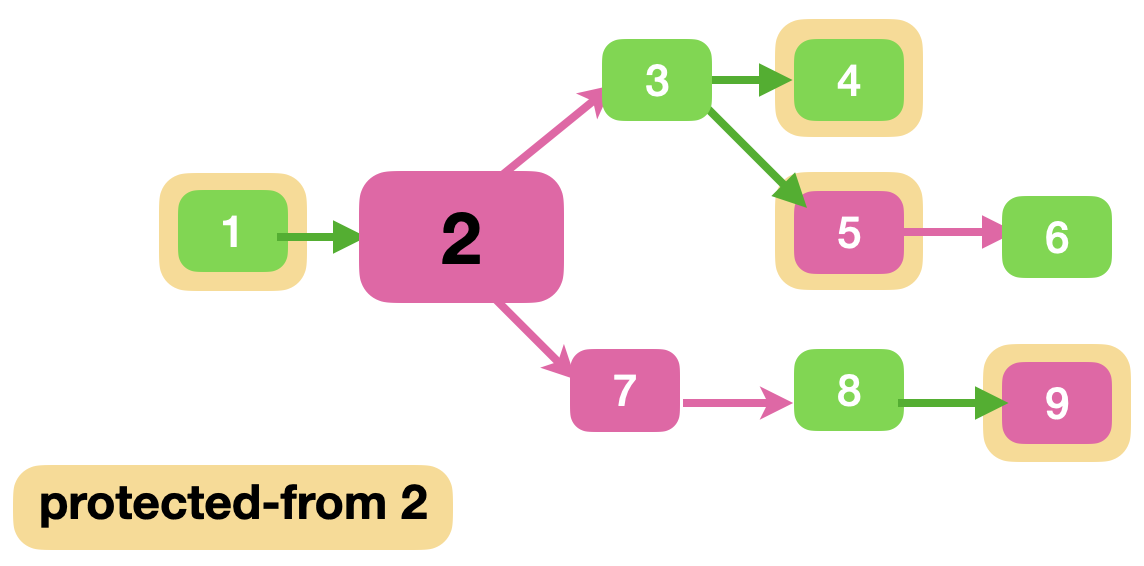
\includegraphics[width=\linewidth]{diagrams/prfC.png}
} 
&
\resizebox{4.5cm}{!}{
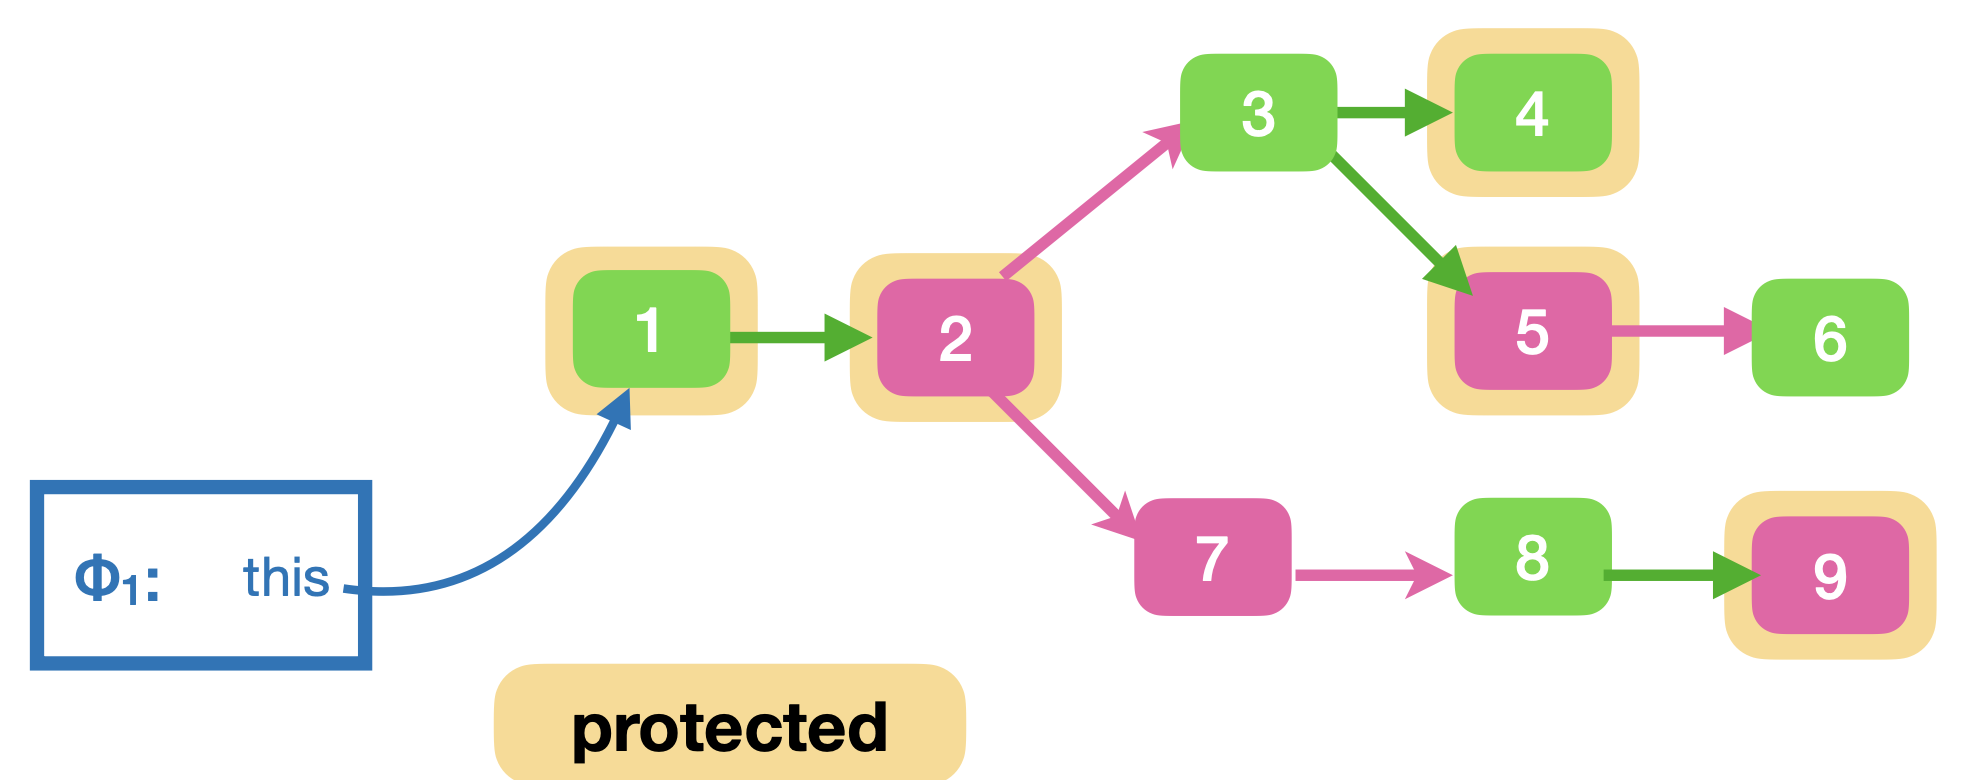
\includegraphics[width=\linewidth]{diagrams/prtFirst.png}
}
&
\resizebox{4.5cm}{!}{
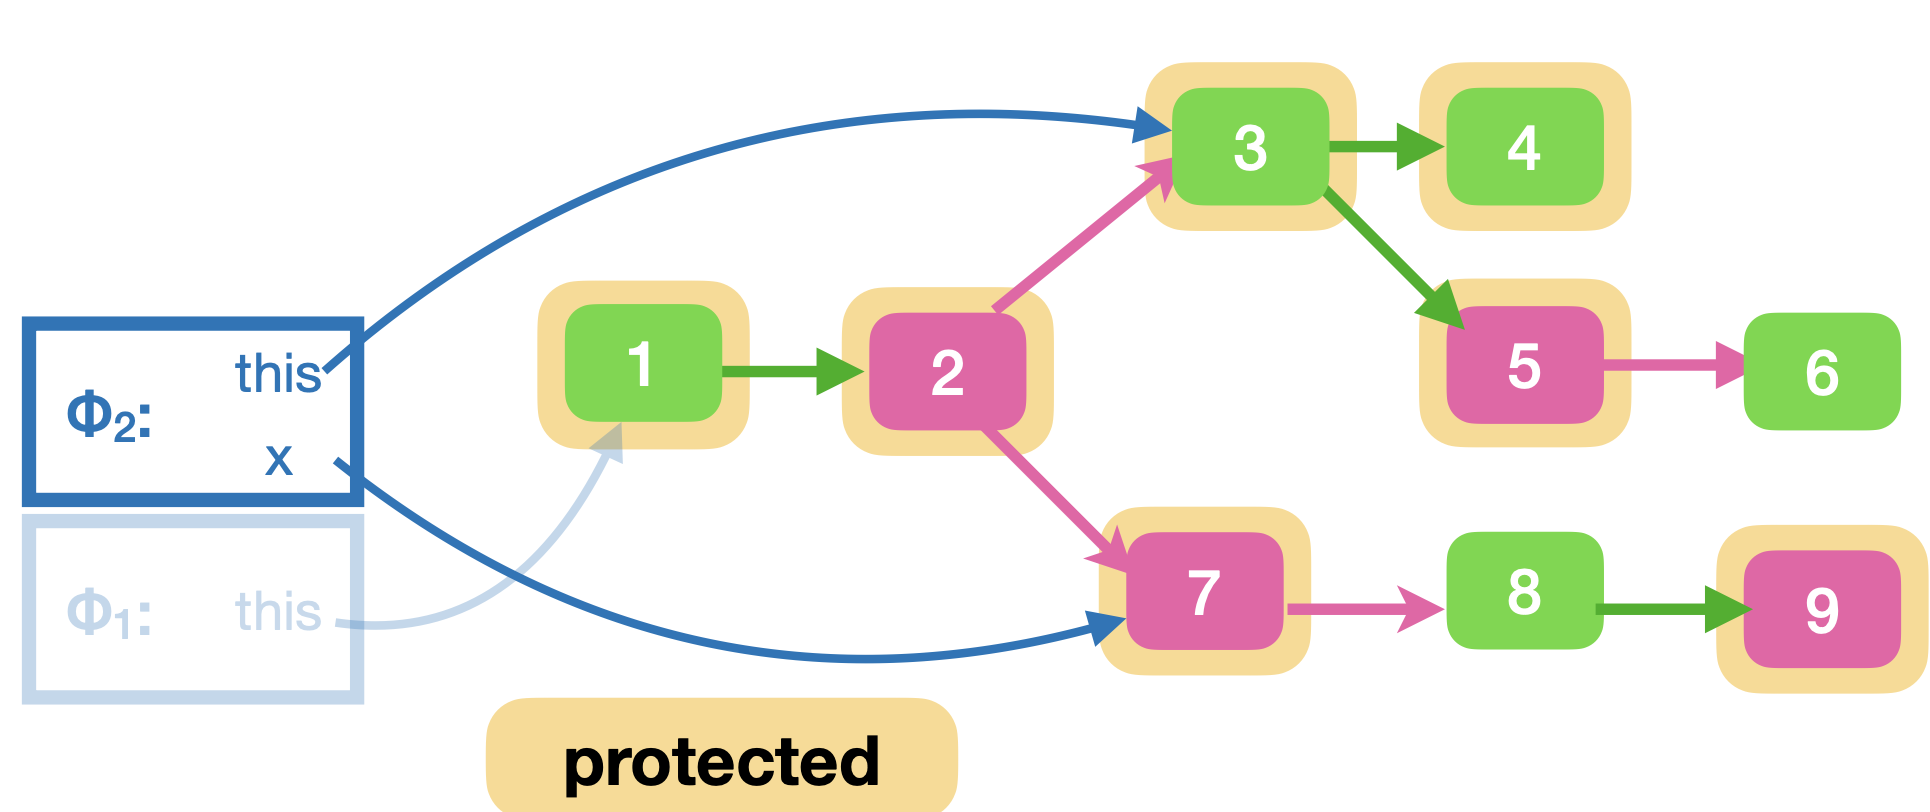
\includegraphics[width=\linewidth]{diagrams/prtSecond.png}
}
\\
\hline
protected from object $o_2$
&
protected  with top frame $\phi_1$
&
protected  with top frame $\phi_2$
\\
\hline \hline
\end{tabular}
\caption{Protected from and Protected. Pink and green squares are external and internal objects, respectively. Connecting straight arrows  indicate fields. Blue boxes are frames on the stack. Protected objects are  highlighted in yellow. 
 The left pane shows a heap with objects $o_1$-$o_9$.
 Here  $o_1$, $o_4$, $o_5$ and $o_9$ 
are protected from $o_2$. 
 The middle pane {shows the same heap and a stack with frame  $\phi_1$} whose receiver,   \prg{this},  points to $o_1$. Here 
 $o_1$, $o_2$, $o_4$, $o_5$ and $o_9$  are protected. 
 The right pane {shows the same configuration, but after pushing frame  $\phi_2$}, whose receiver,  \prg{this},  and local variable, \prg{x}, point to $o_3$ and  $o_7$, respectively.
 Here $o_3$ and $o_7$ are protected, in addition  to  the objects protected in the previous pane.
}
   \label{fig:ProtectedBoth}
 \end{figure}
 

\subsection{2$^{nd}$ Challenge: Specification of tamed effects}
\label{sect:approach:scoped}
How can we express the guarantee that effects are \tamed?  
 In particular, when such effects can be the outcome of the execution of more than one method? 
 Traditional,  {per-method} PRE/POST conditions {cannot guarantee} %specifications cannot express guarantees
  that two or more of our methods won't interact to produce an untamed effect. 
We build on the concept of history invariants \cite{liskov94behavioral,usinghistory,Cohen10} and define

\begin{description}
\item[{Scoped invariants}]  
{$\TwoStatesN  {\overline{x:C}}  {A}$} expresses that if a {state} $\sigma$ 
 has objects $\overline x$ of class $\overline C$, and satisfies $A$, then all $\sigma$'s \emph{scoped  future  states} will  {also} satisfy  {$A$}. 
The scoped future contains all % \sdN{future} 
 states which can be reached through any steps, including further method calls and returns, but stopping before returning  from the call active in $\sigma$ \footnote{{Here lies the difference to history invariants, which consider \emph{all} future states, including returning from the call active in $\sigma$.}}  --  \cf Def  \ref{def:shallow:term}.
{For} $\sigma$ and its scoped future   we only consider external states -- \cf Def \ref{def:necessity-semantics}.
\end{description}

    
\label{s:bank}



\begin{example}
\label{s:bankSpecEx}
The following scoped invariants\\
$\strut \SPSP\ \ \   S_1\ \  \triangleq \ \ \TwoStatesN {\prg{a}:\prg{Account}}  {\inside{\prg{a}}} $ 
\hspace{1.1cm}
$\strut  \SPSP\ \ \   S_2\ \  \triangleq \ \ \TwoStatesN  {\prg{a}:\prg{Account}}  {\inside{\prg{a.key}}} $ 
% \\
%$\strut  \SPSP   S_3\ \  \triangleq \ \ \TwoStatesN {\prg{a}:\prg{Account},\prg{b}:\prg{int}}  {\inside{\prg{a}} \wedge \prg{a.\balance}=\prg{b}}  $
\\
$\strut  \SPSP\ \ \   S_3\ \  \triangleq \ \ \TwoStatesN{ \prg{a}:\prg{Account},\prg{b}:\prg{int} } {\inside{\prg{a.key}} \wedge \prg{a.\balance} \geq \prg{b} } $ 
% \end{tabular}
%}

\noindent
%specifications
 guarantee that   accounts are not leaked  ($S_1$), \ \ keys are not leaked  ($S_2$), \ \ the balance does not decrease unless there is unprotected access to the key  ($S_3$).
 % $\strut  \SPSP  S_1$:\   accounts are not leaked,  \hspace{1.1cm}
%$\strut   \SPSP S_2$:\    keys are not leaked,\\
%%$\strut \SPSP  S_3$:\  the balance is not modified unless there is unprotected access to the account,  \\%while 
%$\strut \SPSP  S_3$:\   the balance does not decrease unless there is unprotected access to the key.  
%
\end{example} 


 
 \vspace{.05cm}

 
\noindent
{\textbf{\sdN{Scoped invariants are} \emph{conditional}}:}  They ensure that assertions are \emph{preserved}, but unlike object invariants, they do not guarantee that they always hold.
\ \Eg   \prg{buy} cannot assume $\inside{a.\prg{key}}$ holds on entry, but   guarantees that if it holds on entry, then  it will still hold on exit.

 
 \begin{example}
 We   use the features from the previous section to specify methods. 

{\sprepost
		{\strut \ \ \ \ S_4} 
		{   \protectedFrom{\prg{this}.\prg{\myAccount}.\prg{key}} {\prg{buyer}} \wedge \prg{this}.\prg{\myAccount}.\prg{\balance}=b
		 }
		{\prg{public Shop}} {\prg{buy}} {\prg{buyer}:\prg{external}, \prg{anItem}:\prg{Item} }
		{ 
		  %\protectedFrom{\prg{this}.\prg{\myAccount}.\prg{key}} {\prg{buyer}} \wedge 
		  \prg{this}.\prg{\myAccount}.\prg{\balance}\geq b
		 }
}

\noindent
$S_4$  guarantees that if the % account's 
key was protected from \prg{buyer} before the call, then the balance will not decrease. %SD is shorter, but I hope ckear eniugh  \prg{buy} will not decrease the %shop's account  balance. 
 It does \emph{not} guarantee \prg{buy} will only be called when $\protectedFrom{\prg{this}.\prg{\myAccount}.\prg{key}} {\prg{buyer}}$ holds. 
As a  public method,  \prg{buy}  can be invoked by external code that ignores all specifications.
\end{example}

% \vspace{.05cm}

\begin{example}
We illustrate the meaning of our specifications  using three  versions of a class \prg{Account}  from  \cite{OOPSLA22} 
as part of our internal module \Mshop. 
To differentiate, we rename \Mshop  as $\ModA$,  $\ModB$, or $\ModC$. 
All use the same \prg{transfer} method for withdrawing money.
%All use the same method \prg{transfer} to  withdraw money, only when supplied with the key.
%\forget{All versions {use the same method \prg{transfer} to} allow  withdrawal of money, only when supplied with the key to the account.
%All use the same method \prg{transfer} to  withdraw money, only when supplied with the key.}
% removed class Key -- it does not need to be internal 
\begin{lstlisting}[mathescape=true, language=Chainmail, frame=lines]
module $\ModA$      
  class Shop   ... as earlier ...
  class Account
    field blnce:int 
    field key:Key
    public method transfer(dest:Account, key':Key, amt:int)
       if (this.key==key')   this.blnce-=amt; dest.blnce+=amt
     public method set(key':Key)
       if (this.key==null)  this.key=key'
\end{lstlisting}

Now consider  modules \ModB and \ModC which differ from \ModA only in their \prg{set} methods. Whereas \ModA 's key is immutable, \ModB allows any client to reset an account's key at any time, and \ModC requires the existing key in order to change it.
  

\begin{tabular}{lll}
\begin{minipage}[b]{0.40\textwidth}

\begin{lstlisting}[mathescape=true, language=Chainmail, frame=lines]
$\ModB$
public method set(key':Key)
  this.key=key'
\end{lstlisting}
\end{minipage}
&\ \ \  \ \   &%
\begin{minipage}[b]{0.48\textwidth}
\begin{lstlisting}[mathescape=true, language=chainmail, frame=lines]
$\ModC$
public method set(key',key'':Key)
  if (this.key==key')  this.key=key''
\end{lstlisting}
\end{minipage} 
\end{tabular}

{Thus, in all three modules, the key is an object capability which \emph{enables} the withdrawal of the money. 
Moreover, in $\ModA$ and $\ModC$, the key
{is a capability} used to  \emph{tame} withdrawal of money, preventing those without it from getting the money from the account.}
Crucially,  in $\ModB$ the key \emph{does not tame} withdrawal of money.
Using $\ModB$, it is possible to start in a state where the account's key is unknown, modify the key, and then withdraw the money. 
Code  {such as}
\\ 
$\ \strut \hspace{.2in} $ \prg{k=new Key;  acc.set(k); acc.transfer(rogue\_accnt,k,1000)} 
\\ 
is enough to drain  \prg{acc} in \ModB without knowing the \password.\footnoteSD{CAREFUL: we had 
$\ \strut \hspace{.01in} $ \prg{an\_account.set(42); an\_account.transfer(rogue\_accnt,42)} but this was type incorrect!}
 %
% \emph{Emergent behaviour} is key here: 
Even though % the method 
\prg{transfer} in  \ModB is ``safe'' when considered in isolation, it is not safe when considered in conjunction with other methods from the same module. 

Our  specifications  rule  out \ModB while permitting \ModA and
\ModC:
No module  satisfies $S_1$. Modules $\ModA$ and $\ModC$ satisfy $S_2$ and $S_3$, while $\ModB$ satisfies neither $S_2$ nor $S_3$.
\end{example}
 
\forget{% for the time being at least
{ \noindent
 Our specifications are  in terms of the complete module, rather than per-method.
 They talk about externally observable effects (\eg the key stays protected), 
 % the account's balance may increase), 
 rather than about  individual methods (\eg\, \prg{set}). %  or \prg{transfer}).
{Thus,   they can characterize  any 
module with  accounts which have a % {\textit{implementation}} of a bank account with a 
 \balance~and a \password -- even as ghost fields --}  irrespective of the API offered.
} }% , services  exported, or  dependencies on other parts of the system.\footnoteSD{does this come from OOPSLA? if so we need to rephrase}
%\notesep
%Adherence to   specifications is not monotonic:
%{Eg, while  \ModA satisfies $S_3$, the addition of \prg{set} lead to \ModB, which does not.}
%% Adding a method to a module does not necessarily preserve such adherence,
%% \eg adding method \prg{set} in module \ModB breaks 
%%SD removed the below. When we changed the invaraints to have the same assertion re and post it no longer hel
%\forget{, and while separate methods may adhere to a  specification, their combination does
%not necessarily do so. 
%{For example, \ModB's  \prg{tansfer} and \prg{set} satisfy $S_3$, but their interplay does not.}
%%In this sense, and, similar to OOPSLA'22, our  specifications capture a module's \emph{emergent behaviour}. 


  
  \subsection{3$^{rd}$ Challenge:  A Hoare logic} %  for external calls} %  (using scoped invariants)}
 \label{sec:howThird}


 
 \vspace{.1cm}
 
We now move to the  verification of $S_4$. 
The challenge is how to reason  about the external call on line 8. %, even though we do not have a specification for \prg{pay}
% the  {called method}, we know that the effects of the call are tamed according to the module's scoped invariants. 
% SD BELOW is wrong. left just in case we want to adapt ir.
% That is expressed in the  simplified Hoare rule below -- \cf. Fig.\ref{f:external:calls}. 
% 
%  $\inferruleNoName  
% 	{ 
%   	   {\TwoStatesN {\overline {x:D}} {A}}\ \   \mbox{is part of $M$'s specification}
%        }
%	{   \triple { \    { \external{y_0}} \,     \wedge \,  \overline{x:D}\  \wedge\  A\ }  
%						{ \ u:=y_0.m(y_1,.. y_n)\    }
%						{ \    A  \ }
%						\  \  ...
%         }
%$
%
%\vspace{.05cm}
% 
% Now  revisit the external call from line 9 in Section \ref{sec:shop}. Our argument is that 
We aim to establish a Hoare triple of the form:
 \\
$\strut \ \ \ \ \ \ \ \ \ \ \  \{\  \ { \external{\prg{buyer}}} \ \wedge\ {\protectedFrom {\prg{this.\myAccount.key}} {\prg{buyer}}\ \wedge\ {\prg{this.\myAccount.\balance}}= b    }\ \  \}$\\
$\strut \ \ \ \ \ \ \ \ \ \ \   \ \ \ \ \ \ \ \ \ \ \ \ {\ \prg{buyer.pay(this.accnt,price)}   \ } $\\
$\strut \ \ \ \ \ \ \ \ \ \ \  \{\  \ \  {\prg{this.\myAccount.\balance}} \geq  b \  \  \}$ 
\\
The intuitive reasoning is as follows: if the shop's account's key is protected from \prg{buyer} (A from earlier), and the module satisfies $S_3$ (B), then after the call, the account's balance will not decrease (C).
%
However, application of $S_3$ is not straightforward. 
%While $S_3$ preserves ${\inside{\prg{a.key}}} \wedge ...$,
%Application of $S_3$ 
It requires ${\inside{\prg{a.key}}} \wedge ...$,  but  the call's precondition only guarantees $\protectedFrom{\prg{this.\myAccount.key}}{\prg{buyer}}$. 
%To apply $S_3$, we would need to know ${\inside{\prg{this.\myAccount.key}}}$, but we only know $\protectedFrom{\prg{this.\myAccount.key}}{\prg{buyer}}$.


%, while we  need the stronger property  ${\inside {\prg{this.\myAccount.key}}}$. 

While we do \susan{not} know whether \prg{a.key} is protected during  execution of \prg{buy}\footnote{For instance, one of the clients may have access to it.}, we can be certain it is protected during execution of \prg{pay}.  This is so, because the objects accessible during \prg{pay} are those visible from its arguments (\ie \prg{buyer} and \prg{price}).
% \footnote{Generally, more objects are protected from the viewpoint of the called function than from that of the caller -- \cf  Fig. \ref{fig},}

%To express this difference, 
We define the adaptation operator $\FIXSymbolA$, which translates an assertion from the viewpoint of the called function to that of the caller. 
Specifically, $\PushAS y A$ ensures that $A$ holds when the variables $\overline{y}$ (where $\overline{y}$ stands for $y_1, ..., y_n$) have been pushed onto a new frame. 
For example, $\PushAS y {(\inside \re)} = \protectedFrom \re {\overline{y}}$ for any term $\re$ (see  \susan{Def. \ref{def:chainmail-protection-from}})
 and Lemma \ref{lemma:push:ass
}).
%
In this case, we have:\\  {\small{$\strut \ \ \ \PushASLong {\{\prg{buyer},\prg{price}\}}  {(\inside {\prg{this.\myAccount.key}})}$
 \ = \  $\protectedFrom {\prg{this.\myAccount.key}} {(\prg{buyer},\prg{price})}$.}}
 \\
 and with this, we \emph{can} apply $S_3$.
 %
 {Below  a  Hoare logic rule  dealing with external calls - \cf. Fig.\ref{f:external:calls}.} % where $\overline y$ stands for $y_1$,,, $y_n$ -
 
 $\inferruleNoName  
 	{ 
   	   {\TwoStatesN {\overline {x:D}} {A}}\ \   \mbox{is part of $M$'s specification}
        }
	{   \triple { \    { \external{y_0}} \,     \wedge \,  \overline{x:D}\  \wedge\  {\PushASLong {(y_0,\overline y)}{A}} \ }  
						{ \ u:=y_0.m(\overline y)\    }
						{ \    {\PushASLong {(y_0,\overline y)}{A}}  \ }
						\  \  ...
         }
$

 
 
 
%   \subsection{4$^{th}$ Challenge: A Hoare Logic for Proving that modules adhere to specifications} %  (using scoped invariants)}
%
% We now revisit the meaning of scoped invariants: 
%  {$\TwoStatesN  {\overline{x:C}}  {A}$} expresses that if an external {state} $\sigma$ 
%% with objects $\overline x$ of class $\overline C$ 
% satisfies $\overline {x:A} \wedge A$, then all its \emph{scoped} external future  states will  {also} satisfy  {$A$}. 
%\Eg if $\sigma$ was an external state executing a call to \prg{Shop::buy}, then a \emph{scoped} external future  state
% could be an external state reachable 
%after the return from \prg{Shop::buy}, but could also be reachable
%during execution of the external call \prg{pay}.
%This means that we are  interested in the states before %and after a method (or statements)
%statements, \emph{but  also}  in the external states reachable \emph{during} execution of these statements. 
%%of that method (or statements).
%To accommodate this, we extend   traditional Hoare triples to quadruples of  form\\
% $\strut \ \hspace{4cm} \quadruple {A} {\, stmt\, }{A'} {A''}$\\  
% promising that if a state satisfies $A$ and executes $stmt$, any terminating state will satisfy $A'$, and 
% and  any intermediate external states reachable during execution of $stmt$ satisfy    $A''$ -- \cf Def. \ref{def:hoare:sem}.
%% same as above, but ugly line break:
%% terminating execution of $stmt$ in  states satisfying $A$  reaches    final states satisfying $A'$, and any intermediate external states reachable during execution of $stmt$ satisfy    $A''$ -- \cf Def. \ref{def:hoare:sem}.
%
%\vspace{.05cm}
%
%The Hoare logic rule from earlier dealing with external calls is:
% 
% $\inferruleNoName  
% 	{ 
%   	   {\TwoStatesN {\overline {x:D}} {A}}\ \   \mbox{is part of $M$'s specification}
%        }
%	{   \quadruple { \    { \external{y_0}} \,     \wedge \,  \overline{x:D}\  \wedge\  {\PushASLong {(y_0,\overline y)}{A}} \ }  
%						{ \ u:=y_0.m(\overline y)\    }
%						{ \   {\PushASLong {(y_0,\overline y)}{A}}  \ }
%						{\  A  \ }
%         }
%$

\vspace{.4cm}

To develop our logic, we   take  a  Hoare logic %of  triples, 
which does not {have} the concept of protection.
%We then extend this logic as follows: We define an embedding into our quadruples. 
%and allow method specifications which also talk about intermediate external states.
We  extend it through % substructural rules, and 
rules talking about protection, and internal and external calls 
-- \cf Figs. \ref{f:underly} -  \ref{f:calls}. % \ref{f:wf}.
A module is well-formed, if  its invariants are well-formed,    its public methods preserve   its invariants, and  all  methods satisfy their specifications - \cf  Fig.  \ref{f:wf}.
An invariant is well-formed if   it is \emph{encapsulated}, \ie can only be invalidated by internal code
-- \cf Def. \ref{d:encaps}. 
A method preserves an assertion   if it preserves it   from pre- to  post-states and also to any intermediate external state.
 Our extension preserves soundness of the  Hoare logic --  \cf   
 Thms.  \ref{l:triples:sound},  \ref{thm:soundness}.




% \vspace{.05cm}
%A module is well-formed, if  its invariants are well-formed,    its public methods preserve   its invariants, and  all  methods satisfy their specifications - \cf  Fig.  \ref{f:wf}.
%% 
%An invariant is well-formed if   it is \emph{encapsulated}, \ie can only be invalidated by internal code
%-- \cf Def. \ref{d:encaps}. 
%A method preserves an assertion   if it preserves it   from pre- to  post-states and also to any intermediate external state.

%\vspace{.05cm}
%%  \se{!!!WE HAVE REMOVED S\_3!!! I CAN REMOVE THE MENTION HERE}
%%\sd{Good catch! Replace with $S_2$ Note that I removed the next paragraph, though.}
%
%\Eg to prove  that method \prg{Shop::buy} satisfies  {$S_2$}  we  need to prove:
%\\
% {\footnotesize{
%%$\strut \ \ \ \ \ \ \ \ \ \ \ \quadruple {A_1  \wedge \inside{\prg{a}} } {\ stmt\_b  \ } {\inside{\prg{a}}} { \inside{\prg{a}}} $
%%\\
%%$\strut \ \ \ \ \ \   \ \  \quadruple {A_1  \wedge  \inside{\prg{a.\password}} } {\  stmt\_buy  \  } {\inside{\prg{a.\password}}}  {\inside{\prg{a.\password}}}$
%%\\
%$\strut \ \ \ \ \ \  \ \  \ \ \   \quadruple {A_1  \wedge  \inside{\prg{a.key}} \wedge  \prg{a.\balance}\!=\!{\prg{b}} } {\   stmt\_b  \  } {\inside{\prg{a.key}} \wedge  \prg{a.\balance}\!=\!\prg{b}}   
%                         {  \inside{\prg{a,key}} \wedge  \prg{a.\balance}\!=\!\prg{b} }$
%%\\
%%$\strut \ \ \ \ \ \   \ \   \quadruple {A_2  \wedge  \inside{\prg{a.\password}} \wedge  \prg{a.\balance}\!\geq\!{\prg{b}} } {\  stmt\_buy  \  } {\inside{\prg{a.\password}} \wedge  \prg{a.\balance}\!\geq\!{\prg{b}}}  
%%   { \inside{\prg{a.\password}}\wedge  \prg{a.\balance}\!\geq\!{\prg{b} }}$
%  }}
%\\
%%and similar for {$S_3$}. Here we used   
%with  $A_1 \triangleq $ % {\footnotesize{
%{{\prg{this}:\prg{Shop}, \prg{buyer}:\prg{external}, \prg{anItem}:\prg{Item}, \prg{a}:\prg{Account}$
%$, \prg{b}:\prg{int}}} and $stmt\_b$   short for  the body of \prg{buy}.
% 
%% \vspace{.2cm}
%%Quadruples are also used in method specifications, \eg we specify \prg{transfer} through
%%\\
%%$\strut \ \ \ \ \ \  \ \  \ \ \  { \mprepostLongN {A_3}{\prg{public}\ \prg{Account}}{\prg{transfer}}{params}{A_4} {true} }$
%%\\
%%with shorthands  $params \triangleq$ \prg{dest:Account}, \prg{key':Key}, \prg{amt:int}, and 
%%$A_3  \triangleq$  $\prg{key'}=\prg{this.\password} \wedge \prg{dest}\neq \prg{this}$
%%$\wedge\, b, b':\prg{int}$
%%$\, \wedge\, \prg{this.\balance}=b$ 
%%$\, \wedge\,  \prg{dest.\balance}=b'$, 
%% and $A_4 \triangleq$  
%% $\prg{this.\balance}=b-\prg{amt} \wedge \prg{dest.\balance}=b'+\prg{amt}$.
%%%For this specification, we need to prove\\
%%%$\strut \ \ \ \ \ \ \ \ \ \ \ \quadruple {\ \prg{this}:\prg{Account}\, \wedge\, params\, \wedge\, A_3  \  } {\ stmt\_{tr}  \ } {A_4} { true} $
%%%\\
%%%where $stmt\_{tr}$ is short for the body of  \prg{transfer}.

\subsection*{Summary}

In our threat model, external objects can execute arbitrary code, invoke any public internal methods, have potentially access to any other external object, and may collude with one another  in any conceivable way.
Our specifications are conditional: they do not guarantee that certain effects will never occur, but they ensure that specific effects will only happen if certain conditions were met prior to the execution of the internal code.
 
The key ingredients of our work are: a) the concept of protection ($\protectedFrom {x} {y}$ and $\inside {x}$), b) the \scoped invariants (${\TwoStatesN {\overline {x:D}} {A}}$), and c) the adaptation operator ($\FIXSymbolA$).
In the remaining sections, we discuss all this in more detail.

% \vspace{0.1cm}
% \noindent
 

 
\footnoteSD{Do we want to talk about the challenges in the proof, and the fact that we reason using sufficient but have necessary in mind.}
\forget{The proof that the extended Hoare logic is sound is interesting, because we are arguing about the soundness of two interrelated systems: 
 the per-statement  Hoare logic, as well as the {entire} module's logic.
Moreover, we need to cater for the possibility that external calls eventually call public methods of the module, which in their turn make external calls etc.
For this we define a new measure of execution ...}

 
 

%%
%%%  

\section{Bits and Bobs: points to make earlier}

\subsection{one}
In the introduction show a method where
\begin{lstlisting}
    void cautious(untrusted : Object, acc: Account){
    PRE acc.passwd PRT-FROM untrusted
    POST acc.passwd PRT-FROM untrusted
     ...
        ext-call does not pass acc.pwd
     ...
   }
\end{lstlisting}

Even external object creation may return an old, preexisting object.
Nevertheless, we are able to prove the above. Make a diagram that has an untrust', which has access to a.pwd. 


\subsection{two}
In our setting, we must deal with the possibility  that any untrusted object may point to any other untrusted object.
Therefore, any reference given to an untrusted object may end up, in principle,  eventually given to all of them.
Therefore if there was an untrusted object $u$ that had reference to $o$,  and we knew that $o$ was protected from $z$ now, we are not
allowed   to deduce that $o$ will still be protected in the "deep" future.
However, if we consider the "shallow" future, we can do better than that.

Namely, if  before an untrusted call with receiver and arguments $\overline z$ we know that $o$ is protected from $\overline z$, and if we know that the internal objects do not leak $o$ to the the external world, then we know that during execution of the untrusted call (and also all nested trusted or untrusted calls), $o$ will be protected (ie no locally accessible external object will obtain direct access), and that after the call, $o$ will still be protected from $\overline z$.

Going back to the discussion where $u$ \kjx{refers}
\st{has an (un-mitigated?)reference} to $o$,  if at the untrusted call
with receiver and arguments $\overline z$, we know that $o$ is
protected from $\overline z$, then this does not preclude
\kjx{$u$ referring to $\overline z$, but it does preclude $\overline
  z$ referring to $u$ -- because if $\overline z \rightarrowtail u$
  then $\overline z \rightarrowtail o$.}
\st{that $u$ has unmitigated access to $\overline z$, but it does precludes that any of  $\overline z$ has unmitigated access to $u$ (because if had, then it would also have had unmitigated access to $o$ itself).}

\subsection{three}
NOTE: JAMES asked Do we need to worry about well-fomedness? Eg what if
we had an assertion $3 \wedge 5 \rightarrow 66$?

  

\subsection{four}
Say that protected-from is a heap property, whereas protected is a
heap-frame property.


\subsection{five}
Say authority implies eventual permission. Ie we want to guarantee that an untrusted object will not get permission to a capability. Lack of eventual permissions bounds authority.


\paragraph{The next sections are organized as follows}
\label{s:semantics}
% In this section we define {the}  \SpecLang specification language.  
We first define an underlying programming language, \LangOO (\S \ref{sub:Loo}).
We then define an assertion language, \AssertLang, which can talk about the
contents of the state, as well as about protection (\S \ref{sub:SpecO}).  Finally, we define the syntax and
semantics of  \SpecLang
specifications (\S \ref{s:holistic-guarantees}).

 


%%
%%

%\renewcommand{\LangOO}{\ensuremath{{\mathcal{L}}_{ul}}\xspace }

\section{The underlying programming language \LangOO}  
\label{sect:underlying}

\subsection{\LangOO syntax and runtime configurations}
\label{sub:Loo} 
{This work} is based on \LangOO, a {small}, imperative, sequential,  class based, typed, object-oriented language. 
 {We believe, however, that the work can easily adapted to any capability safe language with some form of encapsulation. 
Wrt to encapsulation and  capability safety},  \LangOO supports private fields, private and public methods, unforgeable addresses, and no ambient authority (no static methods, no address manipulation).
 It has a simple concept of module with module-private fields and methods, described in Sect. \ref{sect:execution}.
 The definition of \LangOO~ {can be found in   {Appendix \ref{app:loo}.}\footnote{{{The examples in this paper are using  a slightly richer syntax for greater readability.}}}.
 
A \LangOO state, $\sigma$,  consists of a  heap $\chi$, and a   stack. 
{A stack  is a sequence of frames, $\phi_1\!\cdot\!...\!\cdot\! \phi_n$.}
A  frame, $\phi$, consists of a local variable map, and a continuation, \ie a sequence of statements to be executed.
The top frame in a state $(\phi_1\!\cdot\!...\!\cdot\! \phi_n, \chi)$ is $\phi_n$. 


 
\paragraph{Notation} We adopt the following unsurprising notation:
\label{s:notation}
\begin{itemize}
\item
{An object is uniquely identified by the address that points to it. We shall be talking of objects $o$, $o'$ when talking less formally, and of addresses, $\alpha$, $\alpha'$, $\alpha_1$, ...  when more formal.}
\item
$x$, $x'$, $y$, $z$, $u$, $v$,  are variables,  $\va$, $\va'$ ... are either addresses or variables. %, we call these \emph{\atoms}.
\item
$\alpha \in \sigma$ means that $\alpha$ is defined in the heap of $\sigma$, and $x\in \sigma$ means that $x$ is defined in the top frame of $\sigma$.
Conversely,  $\alpha\notin\sigma$ and $x\notin\sigma$ %, and $\va \notin A$ h
 have the obvious meanings.
$\interpret{\sigma}{\alpha}$  is $\alpha$; and $\interpret{\sigma}{x}$  is the value to which  $x$  is mapped in the top-most frame of $\sigma$'s stack, 
and $\interpret{\sigma}{e.f}$ looks up in $\sigma$'s heap the value of $f$ for the object  $\interpret{\sigma}{e}$.
Note that $\interpret{\sigma}{e}$ is not defined when $e$ contains a method call or a ghost field.
\item The  update
$\phi[x \mapsto \alpha]$ is applied to the variable map  of $\phi$,  
and  $\sigma[x \mapsto \alpha]$ is applied to the top frame of $\sigma$.
\item
$A[e/x]$ is textual substitution where we replace all occurrences of $x$ in $A$ by $e.$ 
\item
As usual, $\overline q$ stands for  sequence $q_1$, ... $q_n$, where $q$ can be an address, a variable,    a frame.
Thus,   $\sigma[\overline{x \mapsto \alpha}]$ and $A[ \overline{e/y}]$ 
% applies the substitutions $\overline{x \mapsto \alpha}$ to the top frame.
have the expected meaning.
\item
$\phi.\prg{cont}$ is the continuation of frame $\phi$, and  $\sigma.\prg{cont}$ is the continuation in the top frame.
\item
$text_1 \txteq text_2$ expresses that $text_1$ and $text_2$ are textually equal;  
 $s_1 \txtin   s_2$  means  $s_1 \txteq  s_2$ or  $s_2 \txteq  s_1; s_3$ for some $s_3$, where $s_1$, $s_2$, and $s_3$ are program statements. 
\item
We define the depth of a stack as $\DepthFs {\phi_1...\phi_n} \triangleq n$, For states, $\DepthSt {(\overline \phi, \chi)} \triangleq  \DepthFs {\overline \phi}$.
The  operator $\RestictTo  \sigma k$ truncates the stack up to the $k$-th frame: % from $\sigma$. Namely, 
 $\RestictTo {(\phi_1...\phi_i...\phi_n,\chi)} {i}  \triangleq   (\phi_1...\phi_i,\chi)$
\item
{ $\vs(stmt)$ returns the variables which appear in $stmt$. For example, $\vs(u:=y.f)$=$\{u,y\}$.}
\end{itemize}

  

  
\subsection{\LangOO Execution}
\label{sect:execution}

 \LangOO execution is described by a small steps operational semantics of the shape $\leadstoOrig  {\Mtwo} {\sigma}   {\sigma'}$ 
 -- {\cf Fig. \ref{f:evaluation}.} 
  $\Mtwo$ stands for one or more modules, where a
  module,  $M$, maps class names to class definitions. 
   
{The semantics enforces dynamically a simple form of module-wide privacy: 
Fields may be read or written only if the class of the object whose field is being read or written, and the class of the object which is reading or writing belong to the same module.}
Private methods may be called only if the class of the receiver (the object whose method is being called), and the class of the caller (the object which is calling) belong to the same module.
Public methods may always be called.

The semantics is unsurprising :  
In $\sigma$, the  top frame's continuation contains the statement to be  executed next.  
 Statements may assign to variables, allocate new objects, 
perform field reads and writes on objects, and
 call methods on those objects. 
When a method is called, a new frame is pushed onto the stack; this frame  maps \prg{this} and the formal parameters to  the values for the receiver and other arguments, and the continuation to the body of the method. 
{Methods are expected to store their return values in the variable \prg{res}.}
 When the continuation is {empty ($\epsilon$), the frame is popped and the value of \prg{res}
 from the popped frame  is stored  in the variable map of the top frame.}
%In other aspects, the semantics is unsurprisring.%we return from that call, its frame is  popped, and execution continues in the context of the calling method. 
%The relation $\leadstoOrigStar  {\Mtwo} {\_}   {\_}$  is the reflexive, transitive closure of $\leadstoOrig  {\Mtwo} {\_}   {\_}$ .
Wlog, we also require that, as in Kotlin, method bodies do not assign to formal parameters. 
This simplifies some proofs and gives rise to a well-formedness requirement for states, 
$\models \sigma$, which guarantees that for all frames  on the stack, the actual parameters of a method call in a  caller frame have the same values as the formal parameters in the called frame, \cf Def.  \ref{def:wf:state}. 
From now on we require implicitly that $\models \sigma$.

Fig. \ref{fig:UpSemantics} illustrates  such  ${\leadstoN}$ execution, where we distibguish
  steps within the same  call ($\rightarrow$),\   entering a method  ($\uparrow$),\    returning from a method  ($\downarrow$).
Thus,  $\sigma_8 \rightarrow \sigma_9$ indicates that  $\leadstoOrig {\Mtwo}{\sigma_8}   {\sigma_9} $ is a step within the same call, 
\ $\sigma_9 \uparrow \sigma_{10}$ indicates that $\leadstoOrig {\Mtwo}{\sigma_9}   {\sigma_{10}} $ is a method entry, \ with 
  $\sigma_{12} \downarrow \sigma_{13}$   the corresponding return. 
In general,  $\leadstoOrigStar  {\Mtwo} {\sigma}   {\sigma'}$ may involve  any number of  calls or returns: \eg
 $\leadstoOrigStar  {\Mtwo} {\sigma_8}   {\sigma_{12}}$ involves one call and no return,
while $\leadstoOrigStar  {\Mtwo} {\sigma_{10}}   {\sigma_{15}}$,   involves no calls and two returns.


\begin{figure}[htb]
\begin{tabular}{|c|}
 \hline %  \\ -- this added one vertical space
\resizebox{7cm}{!}{
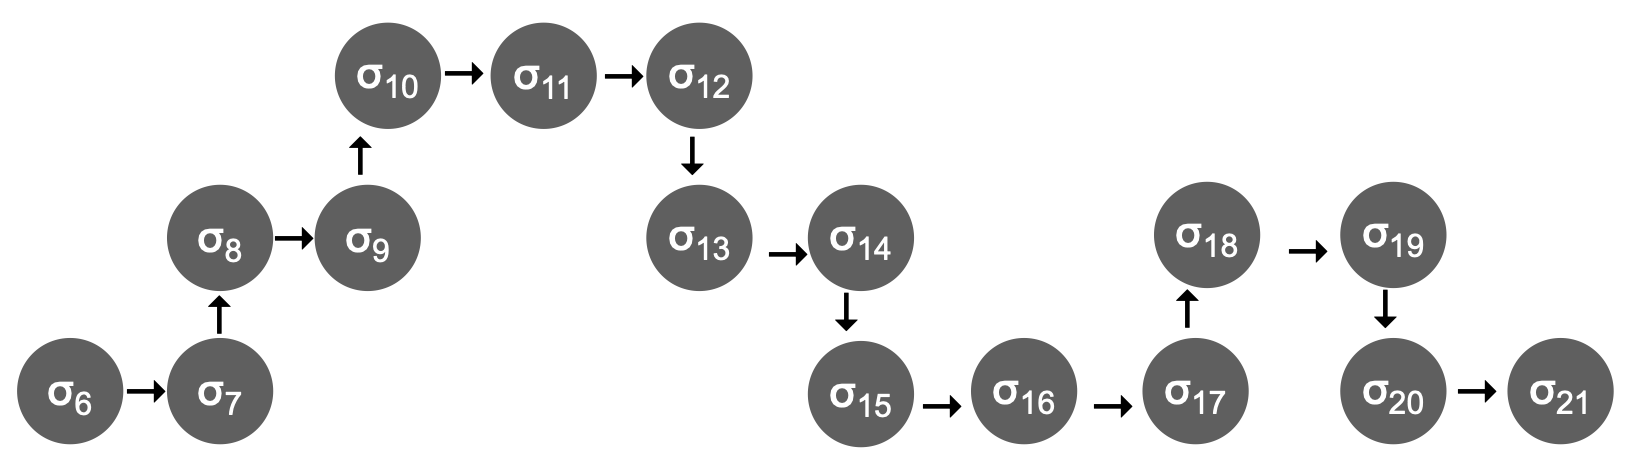
\includegraphics[width=\linewidth]{diagrams/bounded2.png}
} 
 \\
\hline

\end{tabular}
   \caption{$\rightarrow$:\  step within the same method; \ \ $\uparrow$:\    entering a method;\ \  $\downarrow$:  returning from a method}
   \label{fig:UpSemantics}
 \end{figure}
 

\section{Auxiliary concepts}
\label{s:auxiliary}

{To develop the semantics of our assertions language, \AssertLang, we   {define} three auxiliary, {derived}, concepts on  top of  \LangOO: {method calls and returns, scoping}, and reachable objects.}

\subsection{ Method Calls and Returns}
 
Method calls and returns are a fundamental concern for our work. 
They are characterized through pushing/popping   frames on the stack.  
The operator   $ \PushS  {\phi} {\sigma}$ pushes 
frame $\phi$ onto the stack of $\sigma$.
 
 

\begin{definition}
\label{def:push:frame}
Given a state $\sigma$, addresses $\overline \alpha$, a frame $\phi$,  variables or addresses $\overline \va$, we define
\begin{itemize}
\item
 $ \PushSF  {\phi} {\sigma} \ \triangleq \ ({\overline{\phi}\cdot\phi}, \chi)$ \ \ \  if \ \ \  $\sigma=(\overline{\phi}, \chi)$.
%\item
%$ \PushS  {\alpha} {\sigma} \ \triangleq\ \{ \ \sigma' \ \mid\ \exists \phi  \ s.t.\ \ 
%   \sigma'=\PushSF  {\phi} {\sigma}  \ \wedge\    Rng(\phi)=\overline \alpha \ \   \ \}$
%\item
%{$ \PushS  {\va}  {\sigma}\  \triangleq\     \PushS  {\interpret {\sigma} {\va}} {\sigma} $.}
\item
$ \ \sigma\, \popSymbol \ \ \  \triangleq\   { (\overline{\phi}\cdot (\phi_n[\prg{cont}\mapsto stmt][x \mapsto \interpret {\phi_n}{ret}]), \chi)}$ \ \ \  if \\
 $\strut \hspace{1.2cm}  \exists x, y_0, \overline y. [ \ \sigma=(\overline{\phi}\cdot\phi_n\cdot\phi_{n+1}, \chi)$, and $\phi_n(\prg{cont})\txteq x:= y_0.m(\overline y); stmt \ ]$
\end{itemize}
 \end{definition}
\footnoteSD{\red{DO we also need that $\overline \alpha$ were locally reachable in $\sigma$?}}

Consider Fig. \ref{fig:UpSemantics} again: $\sigma_8 = \PushSF  {\phi} {\sigma_7}$ for some $\phi$, and  $\sigma_{15}$=$\sigma_{14} \popSymbol$
--  thus $\sigma_8$ is a called state for 
 $\sigma_7$}, and  $\sigma_{15}$ is the return state from 
 $\sigma_{14}$.
% Note that $\sigma = \sigma' \popSymbol$ iff $\sigma'\!\in\!\PushS  {\phi} {\sigma}$; we can see that 
% Also, 
% $\sigma_{14}\!\in\!\PushS  {\phi'} {\sigma_{15}}$ for some $\overline {\alpha'}$ -- {thus $\sigma_{15}$ is a caller state for  $\sigma_{14}$}.
%\footnote{$\phi'$ may differ from $\phi$, because between $\sigma_8$ and $\sigma_{15}$ there may 
% have been assignments to local variables.} 

  
 \subsection{Scoping}
 \label{sect:bounded}

{The semantics from the earlier section allows arbitrary numbers of method calls and returns. 
\susan{I THINK IT WOULD BE BETTER TO SAY: The semantics from the earlier section does not ensure that method calls and returns match.}
In particular, it is possible to start with a state $\sigma$ and perform more returns than calls --
\eg $\leadstoOrigStar  {\Mtwo} {\sigma_{8}}   {\sigma_{15}}$  in  Fig. \ref{fig:UpSemantics}.
{In the sense of $\leadstoN^* $,  the state $\sigma_{15}$  is one of the future  states for $\sigma_8$.}

 
{For} the purposes of our work, we   need an {additional} notion, of  \emph{scoped} future:  
the scoped future of a state consists of all states which  can be reached through any   
 steps, including method calls and returns, but   {stopping before returning}   
from the method executing in the scoping state}. 
\forget{We say the currently executing method \emph{scopes} the execution.}
Thus, the {scoped} future  of $\sigma_8$   includes only
  $\sigma_9$, $\sigma_{10}$, $\sigma_{11}$, $\sigma_{12}$, $\sigma_{13}$, and $\sigma_{14}$, but \emph{not} $\sigma_{15}$  -- the latter results from returning from $\sigma_{8}$'s top continuation.  
 {Similarly, $\sigma_{18}$ is not in the scoped future of $\sigma_8$, even though the two states have the same stack depth -- between $\sigma_{8}$  and  $\sigma_{18}$ we returned from the top continuation in $\sigma_{8}$.}
 To capture this  notion, we define    {\emph{execution scoped by a state} $\sigma\bd$.}
%To capture this  notion, we define    {\emph{execution scoped by a state} $\sigma\bd$, which allows any steps, except for popping   $\sigma\bd$'s top frame:}

 \renewcommand{\EarlierS}[2]{\DepthSt{#1} \leq \DepthSt{#2}}
 \renewcommand{\NotEarlierS}[2]{\DepthSt{#1} \not\leq \DepthSt{#2}} 
 
\begin{definition}[Scoped Execution] 
\label{def:shallow:term}
% chopped as not needed
% We define relations  $\leadstoBounded  {\Mtwo} {\sigma} {\sigma'}$ as:
$ ~ $ % forcing line break

\begin{itemize}

% OLD VERSION
%\item
% $\EarlierS {\sigma}  {\sigma'} \ \ \ \ \ \  \ \ \ \ \ \ \ \ \ \  \ \ \  \triangleq \ \ % \exists  \psi, \psi', s.t. 
% {\exists  \phi, \phi',\overline \phi, \overline {\phi'},\chi, \chi'.[\  \sigma\!=\!({\overline \phi\cdot \phi},\chi)\, \wedge\, \sigma'\!=\!(\overline \phi\cdot \phi'\cdot \overline {\phi'},\chi')\ ] } $\footnote{Needless to say that   $\overline \phi$ as well as ${\overline {\phi'}}$ may be empty.}
 
% \item
%{ $\leadstoBoundedThree {\Mtwo} {\sigma} {\sigma\bd}  {\sigma'}  \  \   \triangleq \ \    \leadstoOrig {\Mtwo} {\sigma} {\sigma'} \, \wedge\, 
% \EarlierS {\sigma\bd}  {\sigma} \, \wedge\,  \EarlierS {\sigma\bd}  {\sigma'} $}
%\item
% $\leadstoBoundedStarThree  {\Mtwo}  {\sigma}  {\sigma\bd} {\sigma'} \ \ \ \triangleq \ \  \sigma=\sigma' \, \wedge\,  \EarlierS {\sigma\bd}  {\sigma}\  \ \ \vee
% \ \ \ \exists \sigma''.[\ \leadstoBoundedThree  {\Mtwo}  {\sigma}  {\sigma\bd} {\sigma''} \, \wedge\, 
%\leadstoBoundedStarThree {\Mtwo} {\sigma''} {\sigma\bd}  {\sigma'}\ ]$
% \item
%{  $\leadstoBounded  {\Mtwo} {\sigma}   {\sigma'} \ \  \ \ \ \ \   \,   \ \ \ \triangleq \ \ \  \leadstoBoundedThree {\Mtwo} {\sigma} {\sigma}  {\sigma'}$}
%  \item
%{  $\leadstoBoundedStar {\Mtwo}  {\sigma}  {\sigma'}   \ \ \ \ \ \ \,  \ \ \ \  \ \triangleq  \ \ \  \leadstoBoundedStarThree {\Mtwo}  {\sigma}  {\sigma} {\sigma'}$}\ \  
%\item
%  $\leadstoBoundedStarFin {\Mtwo}  {\sigma}  {\sigma'}   \ \ \ \ \  \,  \ \  \ \triangleq  \ \ \  \leadstoBoundedStar {\Mtwo}  {\sigma}  {\sigma'}  \ \wedge\ \
% {\DepthFs \sigma = \DepthFs {\sigma'} \ \ \wedge \ \ \sigma'.\prg{cont}=\epsilon  } $
  \item
{  $\leadstoBounded  {\Mtwo} {\sigma}   {\sigma'} \ \ \   \,   \ \ \ \triangleq \ \ \  \leadstoOrig {\Mtwo} {\sigma} {\sigma'} \, \wedge\, 
 \EarlierS {\sigma}  {\sigma'} $}
  \item
{  $\leadstoBoundedStar {\Mtwo}  {\sigma_1}  {\sigma_n}  \ \ \,  \ \    \ \triangleq  \ \ \  {\sigma_1} = {\sigma_n}\ \ \vee \ \  \exists \sigma_2,...\sigma_{n-1}.\forall i\!\in\! [1..n)[\  \leadstoOrig {\Mtwo}  {\sigma_i}  {\sigma_{i+1}}\  \wedge\  \EarlierS{\sigma_1} {\sigma_{i+1}} \ ]$ }
% \wedge\,  \EarlierS{\sigma_1} {\sigma_n}$}\ \  
\item
  $\leadstoBoundedStarFin {\Mtwo}  {\sigma}  {\sigma'}  \  \,  \ \  \ \triangleq  \ \ \  \leadstoBoundedStar {\Mtwo}  {\sigma}  {\sigma'}  \ \wedge\ \
 {\DepthFs \sigma = \DepthFs {\sigma'} \ \ \wedge \ \ \sigma'.\prg{cont}=\epsilon  } $
 \end{itemize}
\end{definition}


Continue with  Fig. \ref{fig:UpSemantics}.
Here $\EarlierS {\sigma_8} {\sigma_9}$ and thus $\leadstoBounded   {\Mtwo} {\sigma_8} {\sigma_9}$. Also,  {$\leadstoOrig {\Mtwo} {\sigma_{14}}  {\sigma_{15}}$  but  $\NotEarlierS {\sigma_{14}} {\sigma_{15}} $ and therefore   $\notLeadstoBounded  {\Mtwo}  {\sigma_{14}}   {\sigma_{15}}$ --  this step pops  $\sigma_{14}$'s  top frame. 
Finally, even though $\DepthSt {\sigma_8} = \DepthSt {\sigma_{18}}$
%$\sigma_8$ and $\sigma_{18}$ have the same depth of stack 
 and $\leadstoOrigStar {\Mtwo} {\sigma_8}  {\sigma_{18}}$, we have  
 $\notLeadstoBoundedStar {\Mtwo} {\sigma_8}   {\sigma_{18}}$: in 
This is so, because the execution $\leadstoOrigStar {\Mtwo} {\sigma_8}  {\sigma_{18}}$ goes through the step
$\leadstoOrig {\Mtwo} {\sigma_{14}}  {\sigma_{15}}$ and  $\NotEarlierS {\sigma_{8}} {\sigma_{15}} $
 -- this step pops  $\sigma_8$'s top stack frame.

\vspace{.05cm}
Lemma \ref{lemma:orig:to:bounded:front} says, essentially,  that \scoped executions describe the same set of executions as those  starting at an initial state\footnote{An \emph{Initial} state's heap contains a single object of class \prg{Object}, and
its  stack   consists of a single frame, whose local variable map is a mapping from \prg{this} to the single object, and whose continuation is  any statement.
(See Def. \ref{def:initial})}.   
For instance, revisit  Fig. \ref{fig:UpSemantics}, and assume that $\sigma_6$ is an initial state.
We have  $\leadstoOrigStar {\Mtwo} {\sigma_{10}}  {\sigma_{14}}$ and $ \notLeadstoBoundedStar {\Mtwo}  {\sigma_{10}} {\sigma_{14}}$, but also 
%However, because $\sigma_6$ is an initial state, we have 
 $\leadstoBoundedStar  {\Mtwo}  {\sigma_{6}}   {\sigma_{14}}$. %  -- \cf Lemma \ref{lemma:orig:to:bounded}.
% SD chopped as we removed that part of lemma
%Moreover, we have that  $\forall i\in [6..9].\leadstoBoundedStarThree {\Mtwo}  {\sigma_{10}} {\sigma_{i}}  {\sigma_{14}}$ -- part (\ref{otbThree})  from above. 


 \begin{lemma}
\label{lemma:orig:to:bounded:front}
For all modules $\overline M$, state  $\sigma_{init}$  $\sigma$, $\sigma'$, where
$\sigma_{init}$ is an initial state:
% and 
%\ref{def:arising} and the 
%{appendices %of the full paper 
%\cite{necessityFull}).}} 
\begin{itemize} % {enumerate} 
\item 
\label{otbOne}
$\leadstoBoundedStar  {\Mtwo}  {\sigma_{init}} {\sigma'} \ \ \Longrightarrow \  \
\leadstoOrigStar {\Mtwo} {\sigma}  {\sigma'}$
%$\leadstoOrigStar {\Mtwo} {\sigma_{init}}  {\sigma}\ \ \Longrightarrow\ \  \leadstoBoundedStar {\Mtwo}  {\sigma_{init}} {\sigma}$.
\item 
\label{otbTwo}
% This version is older and probably more "convincning" -- SD
%$\leadstoOrigStar {\Mtwo} {\sigma_{init}}  {\sigma}\ \wedge\ \leadstoOrigStar {\Mtwo} {\sigma}  {\sigma'}
$\leadstoOrigStar {\Mtwo} {\sigma_{init}}  {\sigma'} \ \wedge\  \leadstoOrigStar {\Mtwo} {\sigma}  {\sigma'}\ \  \Longrightarrow\ \
\leadstoBoundedStar  {\Mtwo}  {\sigma_{init}} {\sigma'}$.
% This version is older and probably more "convincning" -- SD
%\  \leadstoBoundedStarThree {\Mtwo} {\sigma} {\sigma_{init}} {\sigma'}$.
%there exists a $\sigma_o$, such that $\leadstoBoundedStar {\Mtwo} {\sigma_{init}}  {\sigma_o}$, and
% $\leadstoBoundedStar {\Mtwo} {\sigma_o}  {\sigma}$, and $\leadstoBoundedStar {\Mtwo} {\sigma_o}  {\sigma'}$, and $\leadstoBoundedStar {\Mtwo} {\sigma_o}  {\sigma'}$. More specifically, 
% $\leadstoBoundedStarThree {\Mtwo} {\sigma} {\sigma_o} {\sigma'}$.
%\item
%\label{otbThree}
% $\forall i\!\in\! [0..m).\ \leadstoOrig  {\Mtwo} {\sigma_{i}}  {\sigma_{i+1}}\ \wedge\ \sigma_{init}=\sigma_0$ \\
% % \ \wedge \  \sigma=\sigma_m \ \wedge\ \sigma' =\sigma_n  $ \\
%\strut \hspace{0.5cm} $\ \ \Longrightarrow \ \  \exists k\leq m.[\ \ \ \forall i\leq k.[\  % \leadstoBoundedStar  {\Mtwo}   {\sigma_{init}} {\sigma_i}\ \wedge \ 
%\leadstoBoundedStarThree  {\Mtwo}  {\sigma_m}  {\sigma_{i}} {\sigma_n} ]\ \ \  \wedge \ \ \ 
%% $\\ \strut \hspace{3cm} $
% \forall i> k. [\  \notLeadstoBoundedStarThree  {\Mtwo}  {\sigma_m}  {\sigma_{i}} {\sigma_n}\ ] \ \ \ ]$.
%\end{enumerate} 
\end{itemize}
\end{lemma}
 



\vspace{.05cm}

\sdN{Lemma \ref{l:var:unaffect} says that scoped execution does not affect the contents of variables in earlier scopes.}
and that 
the interpretation of a variable remains unaffected by
scoped execution of statements  which do not mention that variable. % Further lemmas can be found
More  in Appendix~\ref{app:aux}.

\begin{lemma}
\label{l:var:unaffect}
For any modules $\Mtwo$, states $\sigma$, $\sigma'$,  variable $y$, and number $k$:
\begin{itemize}
\item
\label{carInFrame}
\sdN{$\leadstoBoundedStar {\Mtwo}  {\sigma}  {\sigma'}  \ \wedge \ k<\DepthSt \sigma  \ \ \Longrightarrow \ \  \interpret {\RestrictTo \sigma k} y =  \interpret {\RestrictTo {\sigma'} k} y$
}
\item
$\leadstoBoundedStarFin {\Mtwo}  {\sigma}  {\sigma'} \ \wedge \ y\notin \vs(\sigma.\prg{cont}) \ \ \Longrightarrow \ \  \interpret \sigma y =  \interpret {\sigma'} y$
\end{itemize}

\end{lemma}


  \subsection{{{Locally} Reachable  Objects}}

 {A central concept to our work is %object 
protection, which we will define in   Sect. \ref{sect:protect}: It requires that no external locally reachable object  
can have unmitigated access to that object.}
An object $\alpha$ is  \emph{locally reachable}, $\alpha \in  \LRelevantO   \sigma $, if it is reachable from the top frame on the stack of $\sigma$.
 
\begin{definition} We define 
\begin{itemize}
\item
\sdN{$ \LRelevantO   \sigma  \ \ \ \ \ \triangleq \ \  \  \{ \ \alpha \ \mid \ \exists n\!\in\!\mathbb{N}.\exists f_1,...f_n, x. [\ \interpret {\sigma} {x.f_1...f_n} = \alpha\ ]$}
\end{itemize}
\end{definition}

 \begin{figure}[htb]
\begin{tabular}{|c|c|c|}
\hline 
\resizebox{3.5cm}{!}{
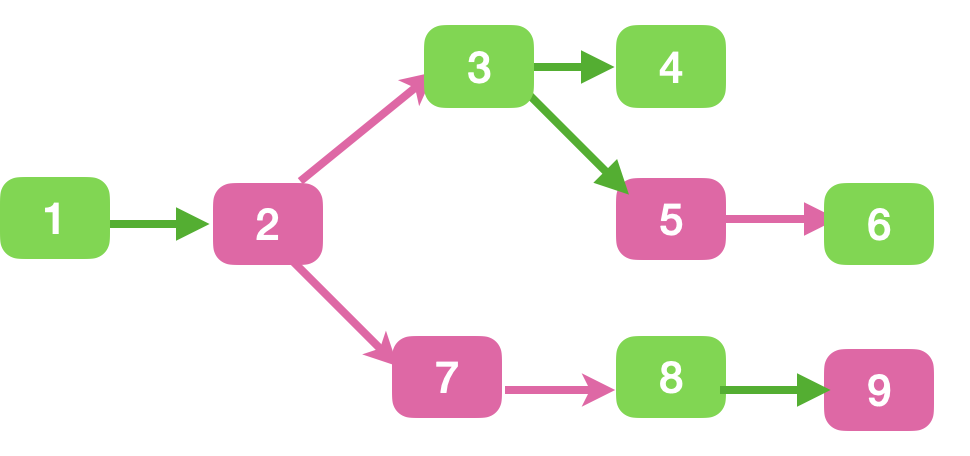
\includegraphics[width=\linewidth]{diagrams/heap.png}
} 
&
\resizebox{5cm}{!}{
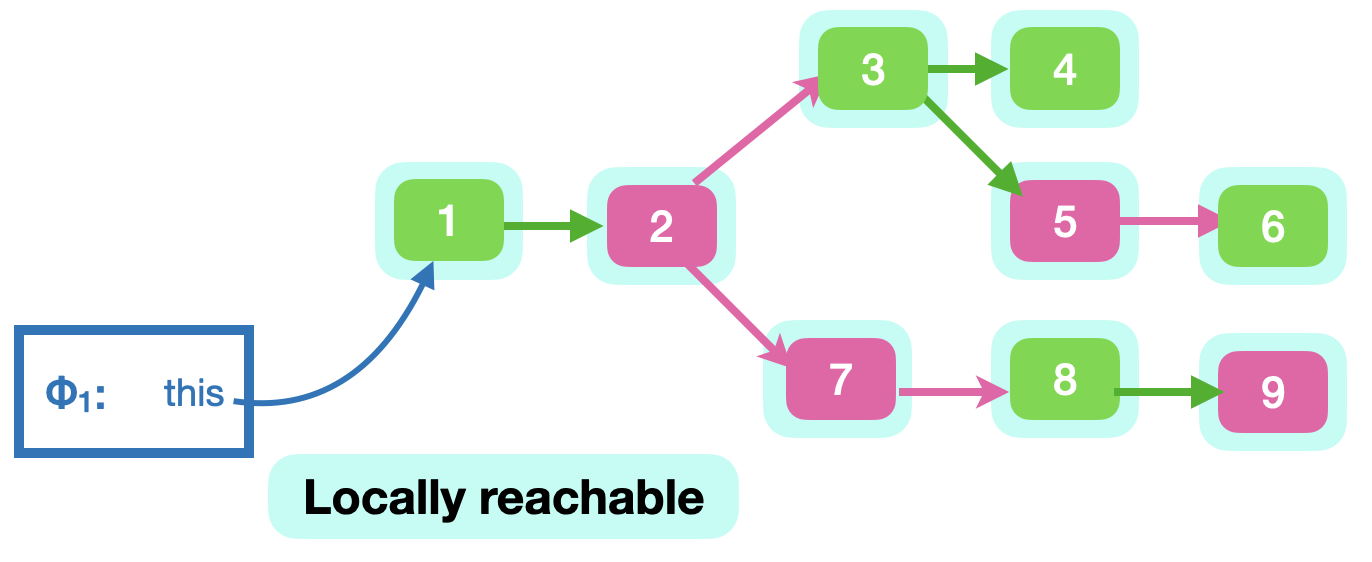
\includegraphics[width=\linewidth]{diagrams/locReachA.png}
} 
&
\resizebox{5cm}{!}{
\includegraphics[width=\linewidth]{diagrams//locReachb.png}
} 
\\
\hline
 a heap
&
Locally Reachable from $\phi_1$
&
Locally Reachable from $\phi_2$
\\
\hline \hline
\end{tabular}
   \caption{A heap, two stacks, and Locally Reachable Objects.
  Distinction  objects into  green/pink  explained later. } % from $\phi_1$ and $\phi_2$. } % n later chapters}
   \label{fig:LReachable}
 \end{figure}

We illustrate these concepts in Fig. \ref{fig:LReachable}:  In the middle pane the top frame is $\phi_1$ which maps \prg{this} to $o_1$; all objects are locally reachable. 
In the right pane the top frame is $\phi_2$, which maps \prg{this} to $o_3$, and $x$ to $o_7$; now $o_1$ and $o_2$ are no longer locally reachable.

Lemma  \ref{lemma:relevant} % describes properties of global reachability. 
says that 
(\ref{oneLR}) any object which is locally reachable right after pushing a frame was also locally reachable before pushing that frame, and 
(\ref{threeLR}) A pre-existing object, locally reachable after any number of scoped execution steps, was locally reachable at the first step.
\footnoteSD{cite "only connectivity begets connectivity"}

\begin{lemma}
\label{lemma:relevant}
\label{lemma:push:N}
For all module sets $\Mtwo$, states $\sigma$, $\sigma'$,   address $\alpha$, and $\overline \alpha$, variables, $x$, $\overline {y}$,:
\begin{enumerate}
\item
\label{oneLR}
\sdN{$ \sigma'\!\in\! \PushS {\alpha} {\sigma}   \ \wedge  \  {\overline \alpha} \subseteq \LRelevantO  {\sigma} 
 \ \  \Longrightarrow\ \ \LRelevantO {\sigma'}\  \subseteq \LRelevantO   {\sigma}$}
\item
\label{threeLR}
\sdN{${\leadstoBoundedStar {\Mtwo}  {\sigma}    {\sigma'}}  \ \  \Longrightarrow\ \ 
dom(\sigma) \cap \LRelevantO {\sigma'} \subseteq   \LRelevantO {\sigma}$
}

\end{enumerate}
\end{lemma}

{Consider Fig.  \ref{fig:UpSemantics}. %, and Fig.  \ref{fig:UpSemanticsBounded}.
Lemma \ref{lemma:relevant}.\ref{threeLR}  promises that any objects locally reachable in $\sigma_{14}$ which already existed in $\sigma_{8}$, were locally reachable in $\sigma_{8}$. However, the lemma is only  applicable to scoped execution, and as 
$\notLeadstoBoundedStar {\Mtwo} {\sigma_8}  {\sigma_{17}}$, 
the lemma does not promise that  objects locally reachable in $\sigma_{17}$ which already existed in $\sigma_{8}$, were locally accessible in $\sigma_{8}$ -- namely it could be that objects are made globally reachable upon method return, during the step from $\sigma_{14}$ to $\sigma_{15}$.}

 
  
 %Thus, if $\sigma_a$ is the result of pushing a frame onto $\sigma_b$, then $\sigma_a\in   \PushS  {\alpha} {\sigma_b}$. 
%{Similarly, if $\sigma_b$ is the result of popping a frame from $\sigma_a$, then $\sigma_a\in   \PushS  {\alpha} {\sigma_b}$.}
 % below Therefore, as 
 %\  (\ref{pushOne}):\  If $\leadstoOrig {\Mtwo} {\sigma}   {\sigma'} $ and
%$\sigma$'s continuation starts with a method call), then $\sigma'$ is the result of pushing a frame with the receiver and arguments onto $\sigma$'s stack. \ 
%%  $\sigma'\!\in\!\PushS   {\alpha} {\sigma}$ then $\sigma'$ is a  \emph{called} state of $\sigma$ --  {a direct successor state of    $\sigma$  after calling a method}. % with receiver and arguments $\overline \alpha$). 
% (\ref{pushTwo}):\  If $\leadstoOrig {\Mtwo} {\sigma}   {\sigma'} $ and $\sigma$'s continuation is the last statement before a method returns, then $\sigma'$   results by popping the top frame % containing   some arguments ($\overline \alpha$) form
% from $\sigma$'s  stack. 
%Finally, (\ref{oneLR}):\
% {entering} the call.
%\kjx{pretty sure we need one other case: (3a) a locally reachable
%  obbject after a call could have been newly created by that call
%  --
%  \red{SD: Thank you for the comment. 
%  (3) is supposed to talk about immediately after entering the call. It was missing an assumption -- in blue. 
%  Please check the text and the maths.}}
 
  
%\footnote{A stronger lemma can be proven:
%% Lemma \ref{lemma:push:N:S} says that % $\pushSymbol$ characterizes  calls and returns. 
%\  (\ref{pushOne}):\  If $\leadstoOrig {\Mtwo} {\sigma}   {\sigma'} $ and $\sigma'\!\in\!\PushS   {\alpha} {\sigma}$ then $\sigma'$ is a  \emph{called} state of $\sigma$ --  {a direct successor state of    $\sigma$  after calling a method}. % with receiver and arguments $\overline \alpha$): \ 
%$\sigma'\in   \PushS  {\alpha} {\sigma}  \ \ \Longleftrightarrow \ \ 
%\exists x, m.[\ \ \sigma.\prg{cont} \txteq x:=y_0.m(y_1,..y_n); \_\ \ \wedge \ \overline \alpha = \overline{ \interpret \sigma y} \ \ ] $
%\\
% (\ref{pushTwo}):\  If $\leadstoOrig {\Mtwo} {\sigma}   {\sigma'} $ and $\sigma\! \in\! \PushS   {\alpha} {\sigma'}$  then $\sigma'$ is a  \emph{caller} state  of $\sigma$ -- {a direct successor  of $\sigma$}  after returning from a method:
% \ \ 
% $\sigma\in   \PushS  {\alpha} {\sigma'}  \ \ \Longleftrightarrow \ \ \exists x, \alpha'.[\ \  \sigma.\prg{cont}\txteq\alpha' \ \ \wedge \ \ \sigma'.\prg{cont}\txteq x:=\alpha';\_ \ \ ] $
% }
  


% \label{s:underlying}
   
\section{Assertions and Specifications -- Syntax and Semantics} %\AssertLang -- the assertion language}
\label{s:assertions}
\label{sub:SpecO}


Our assertions are  %\AssertLang, 
 standard  or  \emph{object-capability}. 
 Standard assertions assert properties of the values of fields, implication, quantification etc, as well as ghost fields  which represent user-defined predicates. 
The  object capability assertions express restrictions of  objects' eventual authority on other objects.

\begin{definition}
\label{def:assert:syntax}
%Expressions, $\re$, 
Assertions, $A$,  are defined as follows:

\label{f:chainmail-syntax}
$
\begin{syntax}
%\syntaxElement{\re}{}
%		{
%		\syntaxline
%				{\prg{true}}
%                                {{\alpha}}
%				{{x}}
%                                {\re.f}
%				{\re.f({\overline{\re}})}
%		\endsyntaxline
%		}
%\endSyntaxElement

\syntaxElement{A}{}
		{
		\syntaxline
				{{\re}}
				{{\re} : C}
				{\neg A}
				{A\ \wedge\ A}
				{\all{x:C}{A}}
				{\external{{\re}}}
 				{\protectedFrom{{\re}} {{\re}}} 
				 {\inside {{\re}}} 
		\endsyntaxline
		}
\endSyntaxElement\\
\end{syntax}
$
%In the above, we expect that
\footnote{Addresses in assertions % may contain addresses; 
as \eg  in  $\alpha.blnce > 700$, %. While addresses make little sense in user-written assertions, they are 
are useful when giving semantics to universal quantifiers 
\cf Def. \ref{def:chainmail-semantics}.(\ref{quant1}), {when the local map changes \eg upon call and return, and in general,} for scoped invariants, \cf Def. \ref{def:necessity-semantics}.}

\vspace{.1cm}

{$\fv(A)$ returns the free variables in $A$; for example, $\fv(a\!:\!Account \wedge \forall b:int.[a.\balance = b])$=$\{ a \}$.} 
% {{Moreover, $\fv(A)$ is defined in the obvious way to to return   the free variables in $A$; for example, $\fv(a\!:\!Account \wedge \forall b:int.[a.\balance = b])$=$\{ a \}$.}}

\end{definition}

\forget{
\noindent
\textbf{NOTES}  \notesep % Extended expressions, $\re$, and therefore also 
 Assertions  may contain addresses; \eg   $\alpha.bal > 700$. 
{While addresses make little sense in user-written assertions, they are useful when giving semantics to universal quantifiers 
\cf Def. \ref{def:chainmail-semantics}.(\ref{quant1}), {when the local map changes \eg upon call and return, and in general,} for two-state invariants, \cf Def. \ref{def:necessity-semantics}.(2).}
\notesep The syntax does  not distinguish between fields and ghost fields. For instance, $\prg{a}.\prg{\balance}$ may, in some modules (\eg in \ModA), be a field lookup, while in others (e.g. when the balance is defined though an entry in a lookup table) may involve executing a ghost function. 
% -  $\external {\re}$ is short for $\neg \internal {\re}$. We use these forms freely in the subsequent text without further definition.
% \footnoteSD{{\textbf{NOTE for us} It also allows assertions like $a1.passwd \neq a2.passwd$, whereas in the past we would have written as $\exists x,y.[\ a1.passwd=x \wedge  a2.passwd=y \wedge x\neq y\ ]$.}} \footnoteSD{{TODO compare with oopsla }}
}


\begin{definition}[Shorthands] 
{We write $\internal{\re}$ for $\neg (\external {\re})$}, and
$\extThis$. resp. {$\intThis$} for $\external{\prg{this}}$ resp. $\internal{\prg{this}}$. %, and $\re:\prg{intl}$ as short for $ \neg \external {\re}}$. 
Forms such as $A \rightarrow A'$,  $A \vee A'$, and $\exists x:C.A$  can be encoded.
%; we use these forms freely in the subsequent text.
% without further definition.
\end{definition}



\label{def:chainmail-semantics-all}
\label{dup:def:chainmail-semantics}
\noindent
Satisfaction  of Assertions by a module and a state is expressed  through \ $\satisfiesA{M}{\sigma}{{A}}$ \  and defined by cases on the shape of $A$, in definitions \ref{def:chainmail-semantics}  and 
 \ref{def:chainmail-protection}.
 {$M$} is used % might need to 
 to look up the definitions of ghost fields, and to find class definitions to determine whether an object is  external.
 
\footnoteSD{say why we split the def into three defs.} 
\noindent
%\textbf{NOTE}  
%{This is not surprising since the goal of this work is to ensure that external modules cannot break our (internal) module's assertions.}
%\footnoteSD{We need to have clarified internal module earlier.} 
%In most cases, satisfaction depends only on the state $\sigma$, but 
% in some cases it also depends on the module $M$: namely execution of extended expressions   
% -- c.f. Def. \ref{def:chainmail-semantics}, cases (\ref{cExpr}),  (\ref{cInternal}). %,  and (\ref{cExternal}) .

\subsection{Semantics of assertions % \AssertLang 
-- first part}
\label{sect:semantics:assert:standard}

To determine satisfaction of an expression, we    use the evaluation relation, $\eval{M}{\sigma}{e}{v}$,
which says that the expression $e$ evaluates
to value $v$ in the context of state $\sigma$ and module $M$.
As expressions in \LangOO may be recursively defined, their evaluation 
need not   % may not necessarily 
 terminate. Nevertheless, the logic of $A$ remains classical because recursion is restricted
to expressions. %, and not generally to assertions.
\footnoteSD{
The semantics of $\hookrightarrow$ {is} unsurprising 
(see {the appendices %of the full paper 
\cite{necessityFull}).}
We have taken this approach from \citeasnoun{FASE}, which also contains a mechanized Coq proof that assertions are classical \cite{coqFASE}. } %Fig.\ref{f:evaluation}).


\begin{definition}[Satisfaction 
of Assertions -- first part] 
\label{def:chainmail-semantics}
We define satisfaction of an assertion $A$ by a % program 
state $\sigma$ with 
 module $M$ as:
\begin{enumerate}
\item
\label{cExpr}
$\satisfiesA{M}{\sigma}{{\re}}\ \ \ \triangleq \ \ \   \eval{M}{\sigma}{{\re}}{\true}$
\item
\label{cClass}
$\satisfiesA{M}{\sigma}{{{\re}} : C}\ \ \ \triangleq \ \ \   \eval{M}{\sigma}{{\re}}{\alpha}\   \wedge \ \class{\alpha} {\sigma}= C$
\item
$\satisfiesA{M}{\sigma}{\neg A}\ \ \ \triangleq \ \ \   {M},{\sigma}\not\models{A}$
\item
$\satisfiesA{M}{\sigma}{A_1\ \wedge\ A_2}\ \ \ \triangleq \ \ \   \satisfiesA{M}{\sigma}{A_1} \   \wedge \ \satisfiesA{M}{\sigma}{A_2}$
%\item
%$\satisfiesA{M}{\sigma}{A_1\ \vee\ A_2}\ \ \ \triangleq \ \ \   \satisfiesA{M}{\sigma}{A_1}\   \vee \ \satisfiesA{M}{\sigma}{A_2}$
\item
\label{quant1}
$\satisfiesA{M}{\sigma}{\all{x:C}{A}} \ \ \ \triangleq \ \ \   
\forall \alpha.[\   \satisfiesA {M}{\sigma} {\alpha:C}  \ \Longrightarrow   \ \satisfiesA{M}{\sigma} {A[\alpha/x]} \ ] $

%\item
%\label{quant2}
%$\satisfiesA{M}{\sigma}{\ex{x:C}{A}}$ \ \ \ iff \ \ \  
% {$\exists \alpha.[\ \GRelevant \alpha \sigma \wedge  \satisfiesA {M}{\sigma} {\alpha:C}  \ \wedge \ \satisfiesA{M}{\sigma} {A[x/\alpha]}\ ]$.} 
%\item
%\label{cInternal}
%$\satisfiesA{M}{\sigma}{\internal{{\re}}}$ \ \ \ iff \ \ \   $\satisfiesA{M}{\sigma}{{{\re}} : C} \ \wedge\ \ C \in M$
\item
\label{cExternal}
$\satisfiesA{M}{\sigma}{\external{{\re}}} \ \ \ \triangleq \ \ \  \exists C.[\ \satisfiesA{M}{\sigma}{{{\re}} : C} \ \wedge \ C \notin M \ ]$
\end{enumerate}
\end{definition}

 
Note that while execution takes place in the context of one or more modules, $\Mtwo$, satisfaction of assertions considers \emph{exactly one} module  $M$ -- the internal module. 
{$M$} is used  to look up the definitions of ghost fields, and to % find class definitions to 
 determine whether objects are  external.

\subsection{Semantics of Assertions - second part}  

\label{sect:protect}
% Long motivation.
% However the motivation from sect 2 shoud be sufficient
%In the object capabilities model \cite{MillerPhD}, \emph{access} to a capability (called a \emph{permission} in \cite{MillerPhD}
% is a necessary precondition  for producing a given effect;  as expressed by the principle that ``authority (to cause an effect) implies eventual permission'' \cite{permissionAuthority}.
%As   in \S \ref{sec:shop}, and also \cite{OOPSLA22}, if no external object has eventual access for a given capability, then the corresponding effect cannot occur.
% Specifically,  we say that $o$ \emph{has eventual access to} $o'$, to mean  that $o$ either currently has or will acquire direct access to $o'$ in the future \cite{permissionAuthority}.
%
%
%
%Given this, it becomes essential to determine whether eventual access exists in a given state. 
%Unfortunately, this determination is undecidable, as it depends not only on the current object graph but also on the program code being executed.
%
%In this work, we over-approximate lack of eventual access through a combination of two properties: one pertaining to the state, and the other to the internal code. 
%The  property pertaining to the state is $\satisfiesA{M}{\sigma} {\inside {\alpha}}$, \ie that   $\alpha$ is \emph{protected},
%\ie that   {no locally reachable external objects have direct access to $o$.}
%% on any path from a locally reachable object to $o$, the penultimate object  is internal. 
%The  property pertaining to the program is that it preserves the protection of   $o$.
%%
%We can see that if $o$ is protected and the internal code preserves its protection, then no external object can gain eventual access to $o$.

In \S \ref{sect:approach:protection} we % discussed the importance of a guarantee that there will be no external access to a capability, and how this can be modelled 
introduced protection -- we will now formalize this concept. % in Def. \ref{def:chainmail-protection-from}.

 An object is protected from another object, $\protectedFrom{{\alpha}} {{\alpha_{o}}}$, if 
the two objects are not equal, and no external object reachable from $a_o$ has a field pointing to  $\alpha$.
This ensures  that any path leading from $\alpha_o$ to $\alpha$ also leads through an internal object.
 

An object is protected,  $\inside{{\alpha}}$,  if no external object reachable from any of the current frame's arguments has a field pointing to $\alpha$, and if the receiver is external, then   $\alpha$ is not the value of any parameter.  
This  ensures that no external objects reachable from the current receiver or arguments have direct access to $\alpha$ -- such direct access
 is either through a field, or by virtue of the receiver having access to all the arguments.
 


 
\begin{definition}[Satisfaction 
of Assertions  -- Protection] 
\label{def:chainmail-protection-from}
\label{sect:semantics:assert:prtFrom}
 \label{def:chainmail-protection}
-- continuing definitions in \ref{def:chainmail-semantics}:
\begin{enumerate}
\item
\label{cProtected}
 $\satisfiesA{M}{\sigma}{\protectedFrom{{\alpha}} {{\alpha_{o}}}}   \ \ \ \triangleq $ 
  \begin{enumerate}
 \item
$\alpha\neq \alpha_0$,
 % \ \ \ \  and 
 \item
$\forall \alpha'.\forall f.[\ \alpha' \in {\Relevant {\alpha_o} {\sigma}} \wedge\   \satisfiesA{M}{\sigma}{\external {\alpha'}} 
\ \ \Longrightarrow \ \  
  \interpret {\sigma} {\alpha_o.f} \neq \alpha     \ ] $.
\end{enumerate}
\item
\label{sect:semantics:assert:prt}
$\satisfiesA{M}{\sigma} {\inside {\alpha}}  \ \ \ \triangleq \ \ \   $
 \begin{enumerate}
\item
 $\satisfiesA{M}{\sigma}{\extThis}\ \ \Longrightarrow\ \ \forall x\!\in\! \sigma.\ \satisfiesA{M}{\sigma}{x\neq \alpha}$,
 \item
$\forall \alpha'.\forall f.[\ \alpha' \in {\LRelevantO {\sigma}} \wedge\   \satisfiesA{M}{\sigma}{\external {\alpha'}} 
\ \ \Longrightarrow \ \  
  \interpret {\sigma} {\alpha_o.f} \neq \alpha     \ ] $.
  \end{enumerate}
\end{enumerate}
Moreover,  \\
$\strut \ \ \ \ \ \  (3) \ \  \satisfiesA{M}{\sigma}{\protectedFrom{{\re}} {{\re_{o}}}}$ $ \triangleq$
$\exists \alpha, \alpha_{o}. [\  \eval{M}{\sigma}{{\re}}{\alpha}\ \wedge\ \eval{M}{\sigma}{{\re_0}}{\alpha_0} \  \wedge \ 
  \satisfiesA{M}{\sigma}{\protectedFrom{{\alpha}} {{\alpha_{o}}}}\   ]$, \\
  $\strut \ \ \ \ \ \ (4) \ \ \satisfiesA{M}{\sigma}{\inside{\re}}$  $\triangleq$
 $\exists \alpha. [\   \eval{M}{\sigma}{{\re}}{\alpha}\ \wedge \   \satisfiesA{M}{\sigma}{\inside{\alpha}} \  ]$. 

 \end{definition} 
 
 We illustrate "protected" and "protected from" in Fig.  \ref{fig:ProtectedBoth} in \S \ref{s:outline},
and    Fig.  \ref{fig:ProtectedFrom} in App. \ref{appendix:assertions}.
%
In general,  $\protectedFrom{{\alpha}} {{\alpha_{o}}}$ ensures that $\alpha_o$ will get access to $\alpha$ only if another object 
 % an internal object 
 grants that access.
Similarly, $\inside \alpha$ ensures that during execution of the current method, no external object will get direct access to $\alpha$ unless some internal object grants that access.
\footnote{This is in line with the motto "only connectivity begets connectivity" from \cite{MillerPhD}.}
Thus, protection together with protection preservation  (\ie no internal object gives access) guarantee
%are sufficient but not necessary conditions for 
lack of eventual external access.  

 
\footnoteSD{JAMES' comment: If is possible that ``we'' do not know the complete heap (eg we only know about the green stuff.) how do we know whether an object is protected. The answer is that we do not know that it is protected, but we do know that our code guarnartees poreservation of protectedness.
}  
 
 \subsubsection*{Discussion} 
Lack of  eventual 
direct access is a central concept in the verification of code with calls to and callbacks  from untrusted code.
% ARGHHH a joke citatiion? \cite{praiseYou}.   
%Unmediated access is essentially \citet{MillerPhD}'s permission: that we have a ``first
%class'' reference to the capability; that we can call any 
%method in the capability's public interface; that we can
%store or save or present the capability to any other
%object to which we've been introduced
%%\footnote{``nobody can ever be introduced in a ball-room''}
It has already been over-approximated in several different ways, \eg
2nd-class \cite{rompf-second-class-oopsla2016,rompf-dont-pop-second-class-ecoop2022}
or borrowed (``2nd-hand'') references
\cite{boyland-promises-icse1998,boyland-aliasburying-spe2001},
 textual modules \cite{OOPSLA22},
information flow \cite{ddd}, runtime
checks \cite{secure-io-fstar-popl2024},
abstract data type exports \cite{vmsl-pldi2023},
  separation-based invariants 
Iris \cite{iris-wasm-pldi2023,cerise-jacm2024},
-- more in  \S~\ref{sect:related}.
In general, protection is applicable in more situations (i.e.\ is less
restrictive) than most of these approaches,
 although more restrictive than the ideal ``lack of eventual access''. 
\footnoteSD{ HER WHAT IT USED TO SAY: the contrapositive ideal that lack of eventual access ensures
lack of effect. Note that ``cannot get direct access'' does not generally imply ``is protected''. 
}





\noindent
\begin{flushleft}
\begin{tabular}{@{}lr@{}}
  \begin{minipage}{.85\textwidth}
   {An alternative definition might consider $\alpha$ as protected from $\alpha_o$, 
if   any path from $\alpha_o$ to $\alpha$ goes through at least one internal object.
With this definition, $o_4$ would be protected from $o_1$ in the heap shown here.
However,  $o_1$ can make a call to $o_2$, and  this call could  return $o_3$. 
Once $o_1$ has direct access to $o_3$, it can also get direct access to $o_4$. 
The example justifies our current definition.  
}
\end{minipage}
& 
\begin{minipage}{.18\textwidth}
\resizebox{2cm}{!}{
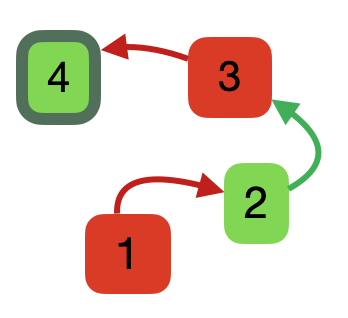
\includegraphics[width=\linewidth]{diagrams/altDef.png}
} 
\end{minipage}
\end{tabular}
\end{flushleft}


%Protection --- \sdN{objects to which external objects may not get %which objects can get 
%unmediated access} % to which other objects 
%---  is  a crucial concept: It enables
%the verification code in the open world, % even in the presence of
%with calls to and callbacks 
%from untrusted code.
%% ARGHHH a joke citatiion? \cite{praiseYou}.   
%Unmediated access is essentially \citet{MillerPhD}'s permission: that we have a ``first
%class'' reference to the capability; that we can call any 
%method in the capability's public interface; that we can
%store or save or present the capability to any other
%object to which we've been introduced
%%\footnote{``nobody can ever be introduced in a ball-room''}
%(compare
%2nd-class \cite{rompf-second-class-oopsla2016,rompf-dont-pop-second-class-ecoop2022}
%or borrowed (``2nd-hand'') references
%\cite{boyland-promises-icse1998,boyland-aliasburying-spe2001}
%which are restricted in some way),
%without reference to some owning class or defining module.
%We discuss alternative designs,
%ranging from overly simplistic textual modules \cite{OOPSLA22},
%information flow \cite{ddd}, runtime
%checks \cite{secure-io-fstar-popl2024},
%abstract data type exports \cite{vmsl-pldi2023},
%to automated separation-based invariants in
%Iris \cite{iris-wasm-pldi2023,cerise-jacm2024},
%in section~\ref{sect:related}.
%In general, protection is applicable in more situations (i.e.\ is less
%restrictive) than most of these approaches,
% \sdN{although more restrictive than the ideal "lack of eventual permission"}. 
%\footnoteSD{ HER WHAT IT USED TO SAY:
%the contrapositive ideal that lack of eventual permission ensures
%lack of effect. Note that ``cannot get direct access'' does not generally imply ``is
%protected''


 


\section{Examples} %\AssertLang -- the assertion language}
\label{s:examples}
\section{Proving that \ModC satisifes \SrobustB}
\label{s:examples}
We now revisit our example from  \S  \ref{s:intro} and \S \ref{s:outline},
and outline a proof that \ModC satisfies \SrobustB. 
A {summary} of this proof has already been discussed in \S \ref{s:approach}.
 A more complex variant of this example that employs   can be found in Appendix \ref{app:examples}.
 \sdN{It demonstrates dealing with modules consisting of several classes some of which are confined, and
 which use ghost fields
 defined through functions; it also demonstrates proofs of assertion encapsulation of assertions 
 which involve reading the values of 
 several fields.} \julian{Mechanised versions of the proofs in both this Section, and Appendix \ref{app:examples}
 can be found in the associated Coq artifact in \prg{simple\_bank\_account.v} and \prg{bank\_account.v} respectively.}
 
 \jm[todo: add reference so \prg{simple\_bank\_account.v} \& \prg{bank\_account.v}]{}
 
Recall that an \prg{Account} includes %a \prg{balance} field, and a \prg{transfer} method, along with any other fields and methods. 
 at least a  field  (or ghost field)  called \prg{balance}, and a method called \prg{transfer}. 

%
 We first rephrase 
\SrobustB to use the $\wrapped{\_}$ predicate.
\begin{lstlisting}[language=Chainmail, mathescape=true, frame=lines]
$\SrobustB$ $\triangleq$ from a:Account $\wedge$ a.balance=bal 
          to a.balance < bal onlyIf $\neg\wrapped{\prg{a.pwd}}$
\end{lstlisting}

We next revisit the   \funcSpec from \S \ref{s:bank} and derive the following 
\prg{PRE}- and \prg{POST}-conditions. The first two pairs of \prg{PRE}-, \prg{POST}-conditions correspond to the first two \prg{ENSURES}
clauses from \S \ref{s:bank}, while the next two pairs correspond to the \prg{MODIFIES}-clause. The current expression in terms
of \prg{PRE}- and \prg{POST}-conditions is weaker than the one in \S \ref{s:bank}, and is not modular, but is
sufficient for proving adherence to  \SrobustB.

\begin{lstlisting}[mathescape=true, frame=lines, language=Chainmail]
$\SclassicP$  $\triangleq$
   method transfer(dest:Account, pwd':Password) -> void  
      (PRE: this.balance$=$bal1 $\wedge$ dest.balance$=$bal2 $\wedge$ this.pwd$=$pwd' $\wedge$ this$\neq$dest
       POST: this.balance=bal1-100 $\wedge$ dest.balance=bal2+100)
      (PRE: this.balance$=$bal1 $\wedge$ dest.balance$=$bal2 $\wedge$ (this.pwd$\neq$pwd' $\vee$ this$=$dest)
       POST: this.balance=bal1 $\wedge$ dest.balance=bal2)
      (PRE: a:Account $\wedge$ a.balance$=$bal $\wedge$ a$\neq$this $\wedge$ a$\neq$dest 
       POST: a.balance=bal)          
      (PRE: a:Account $\wedge$ a.pwd$=$pwd1  
       POST: a.pwd=pwd1)         
\end{lstlisting}


%\begin{figure}[t]
%\begin{lstlisting}[mathescape=true, frame=lines]
%module $\ModC$
%  class Password{}
%  class Account
%    field balance:int
%    field pwd:Password
%    method set(pwd':Password, pwd'':Password):void
%      {if(this.pwd==pwd') 
%         this.pwd := pwd'}
%	method transfer(pwd':Password, destAcc:Account)
%	  {if(this.pwd==pwd' && this.balance > 100)
%	     this.balance := this.balance - 100
%	     destAcc.balance := destAcc.balance + 100}
%\end{lstlisting}
%\caption{Bank Account Module}
%\label{f:ex-bank-short1}
%\end{figure}

%Susan: I changed the label because somewhere (I think in an appendix) there is a f:ex-bank-short and the ref picks it up rather than this one

\subsection{Part 1: Assertion Encapsulation}
\label{s:BA-encap}
The first part of the proof demonstrates that the \prg{balance}, \prg{pwd}, and external accessibility to the password are 
encapsulated properties. That is, for the \prg{balance} to change (i.e. for \prg{a.balance = bal} to be invalidated), or for 
or for the encapsulation of \prg{a.pwd} to be broken (ie for a transition from ${\wrapped{\prg{a,pwd}}}$ to $\neg {\wrapped{\prg{a.pwd}}}$),
internal computation is required. 

We use \sdNr[used to say "a conservative approach to an encapsulation system" but "conservative" here means sound]{a simple encapsulation system}, detailed in \jm[]{Appendix} \ref{s:encap-proof}, 
and provide the proof steps below.
\textbf{\prg{aEnc}} and \textbf{\prg{balanceEnc}} state that 
\jm[]{\prg{a} and \prg{a.balance}} satisfy \sdN{the \textsc{Enc$_e$} predicate. That is, if any objects' contents are to be
looked up during execution of these expressions, then these objects are internal.}
\textsc{Enc}$_e$(\prg{a}) holds because no object's contents is looked up,
while \textsc{Enc}$_e$(\prg{a.balance}) holds because \prg{balance} is a field of \prg{a}, and \prg{a} is
internal.
\\
\begin{figure}[h]
\begin{proofexample}
\proofsteps{\prg{BalEncaps}}
	{\begin{proofexample}
		\proofsteps{\prg{aEnc}}
			{\proofstepwithrule
			{$\proves{\ModC}{\givenA{\prg{a:Account $\wedge$ a.balance=bal}}{\intrnl{\prg{a}}}}$}
				{by \textsc{Enc$_e$-Obj}}
		}
		\endproofsteps
	\end{proofexample}
		}
	{\begin{proofexample}
		\proofsteps{\prg{balanceEnc}}
			{\proofstepwithrule
			{$\proves{\ModC}{\givenA{\prg{a:Account $\wedge$ a.balance=bal}}{\intrnl{\prg{a.balance}}}}$}
				{by \prg{aEnc} and \textsc{Enc-Field}}
		}
		\endproofsteps
	\end{proofexample}
		}
	{\begin{proofexample}
		\proofsteps{\prg{balEnc}}
			{\proofstepwithrule
			{$\proves{\ModC}{\givenA{\prg{a:Account $\wedge$ a.balance=bal}}{\intrnl{\prg{bal}}}}$}
				{by \textsc{Enc$_e$-Int}}
		}
		\endproofsteps
	\end{proofexample}
		}
		{\proofstepwithrule
			{
			$\proves{\ModC}{\givenA{\prg{a:Account $\wedge$ a.balance=bal}}{\encaps{\prg{a.balance=bal}}}}$
			}{by \prg{balanceEnc}, \prg{balEnc}, \textsc{Enc-Eq}, and \textsc{Enc-=}}}
\endproofsteps
\end{proofexample}
\end{figure}


\sdN{Moreover},  \textbf{\prg{balEnc}} states that \prg{bal} satisfies \sdN{the \textsc{Enc}$_e$ predicate}
-- it is an integer, and no object look-up is involved in its calculation.
% used to say
% since bal is an integer, {its} value is constant and may not change, and thus is encapsulated.
\textbf{\prg{balanceEnc}} and \textbf{\prg{balEnc}} combine to prove that the assertion \prg{a.balance = bal} is encapsulated --
%Note: it may seem odd to say that the integer \prg{bal}  { or the address
%\prg{a} is encapsulated};  {but remember that their value cannot change, and thus they
%vacuously sarisfy the definition of encapsulation.}
\sdN{only internal object lookups are involved in the validity of that assertion, and therefore only 
internal computation may cause it to be invalidated.}


\sdN{Using similar reasoning, we} prove that \prg{a.pwd} {is encapsulated} (\textbf{\prg{PwdEncaps}}), and
that \wrapped{\prg{a.pwd}} {is encapsulated} (\textbf{\prg{PwdInsideEncaps}}). 
\sdNr[I chopped the below "That is, if only internal objects have access
to an account's \prg{pwd}, then only internal computation may grant  access to \prg{pwd} 
 to an external object." as it only repeats the definition.]{}

\begin{figure}[h]
\begin{proofexample}
\proofsteps{\prg{PwdEncaps}}
		{\proofstepwithrule
			{
			$\proves{\ModC}{\givenA{\prg{a:Account}}{\encaps{\prg{a.pwd=p}}}}$
			}{by \textsc{Enc$_e$-Obj}, \textsc{Enc-Field}, and \textsc{Enc-Eq}}}
\endproofsteps
\end{proofexample}
\\\begin{proofexample}
\proofsteps{\prg{PwdInsideEncaps}}
		{\proofstepwithrule
			{
			$\proves{\ModC}{\givenA{\prg{a:Account}}{\encaps{\wrapped{\prg{a.balance}}}}}$
			}{by \textsc{Enc-Inside}}}
\endproofsteps
\end{proofexample}
\end{figure}

\sdNr[removing references to Hoare logic.]{}

\subsection{Part 2: Per-Method \Nec Specifications}
\label{s:BA-classical}
Part 2 proves necessary preconditions for each method in 
the module interface. 
%We employ the observation that
%we can build necessary preconditions on top of classical 
\sdN{We employ the rules from  \S \ref{s:classical-proof} which describe how to derive 
necessary preconditions from \funcSpecs.
}
%Hoare logic (\S \ref{s:classical-proof}).

\textbf{\prg{SetBalChange}} uses a 
 \funcSpec and a rule of consequence
% classical Hoare logic
to prove that the \prg{set} method in \prg{Account}
never modifies the \prg{balance}. We then use \textsc{If1-Classical}
and our \Nec logic to prove that if it ever did change (a logical absurdity),
then \prg{transfer} must have been called.
\begin{figure}[htb]
{
	\begin{proofexample}
		\proofsteps{SetBalChange}
			{\proofstepwithrule
				{\hoareEx
						{a, a$^\prime$:Account $\wedge$ a$^\prime$.balance=bal}
						{a.set(\_, \_)}
						{a$^\prime$.balance = bal}
						}
					{by \funcSpec}
			}
			{\proofstepwithrule
				{\hoareEx
						{a, a$^\prime$:Account $\wedge$ a$^\prime$.balance = bal $\wedge$ $\neg$ false}
						{a.set(\_, \_)}
						{$\neg$ a$^\prime$.balance < bal }
						}
					{by 
					\sdN{rule of consequence}} %Hoare logic}
			}
			{\proofstepwithrule
				{\onlyIfSingleExAlt
						{a, a$^\prime$:Account $\wedge$ a$^\prime$.balance=bal $\wedge$ $\calls{\_}{\prg{a}}{\prg{set}}{\prg{\_, \_}}$}
						{a$^\prime$.balance < bal}
						{false}
						}
					{by \textsc{If1-Classical}}
			}
			{\proofstepwithrule
				{\onlyIfSingleExAlt
						{a, a$^\prime$:Account $\wedge$ a$^\prime$.balance=bal $\wedge$ $\calls{\_}{\prg{a}}{\prg{set}}{\prg{\_, \_}}$}
						{a$^\prime$.balance < bal}
						{$\calls{\_}{\prg{a}^\prime}{\prg{transfer}}{\prg{\_, a$^\prime$.pwd}}$}
						}
					{by \textsc{Absurd} and \textsc{If1-}$\longrightarrow$}
			}
		\endproofsteps
	\end{proofexample}
}
\end{figure}

\sdN{Similarly,} in \textbf{\prg{SetPwdLeak}}  we employ \funcSpecs % classical Hoare logic
to prove that a method does not leak access to some data (in this case the \prg{pwd}).
Using \textsc{If1-Inside}, we reason that since the return value of \prg{set} is
\prg{void}, and \prg{set} is prohibited from making external method calls,
no call to \prg{set} can result in an object (external or otherwise) gaining access to the \prg{pwd}.
\begin{figure}[htb]
{
	\begin{proofexample}
		\proofsteps{SetPwdLeak}
			{\proofstepwithrule
				{\hoareEx
						{a:Account $\wedge$ a$^\prime$:Account $\wedge$ a.pwd == p}
						{\prg{res}=a$^\prime$.set(\_, \_)}
						{res != pwd}
						}
					{by \funcSpec}
			}
			{\proofstepwithrule
				{\hoareEx
						{a:Account $\wedge$ a$^\prime$:Account $\wedge$ a.pwd == p $\wedge$ $\neg$ false}
						{\prg{res}=a$^\prime$.set(\_, \_)}
						{res != p}
						}
					{by \sdN{rule of consequence}} % Hoare logic}
			}
			{\proofstepwithrule
				{\onlyIfSingleExAlt
						{$\wrapped{\prg{pwd}}$ $\wedge$ a, a$^\prime$:Account $\wedge$ a.pwd=p $\wedge$ $\calls{\_}{\prg{a}^\prime}{\prg{set}}{\_, \_}$}
						{$\neg \wrapped{\_}$}
						{false}
						}
					{by \textsc{If1-Inside}}
			}
		\endproofsteps
	\end{proofexample}
	}
	\end{figure}
	
In the same manner as \textbf{\prg{SetBalChange}} and \textbf{\prg{SetPwdLeak}}, we also prove
\textbf{\prg{SetPwdChange}}, \textbf{\prg{TransferBalChange}}, \textbf{\prg{TransferPwdLeak}}, and \textbf{\prg{TransferPwdChange}}. We provide their 
statements, but omit their proofs.
\begin{figure}[htb]
{
	\begin{proofexample}
		\proofsteps{SetPwdChange}
			{\proofstepwithrule
				{\onlyIfSingleExAlt
						{a, a$^\prime$:Account $\wedge$ a$^\prime$.pwd=p $\wedge$ $\calls{\_}{\prg{a}}{\prg{set}}{\prg{\_, \_}}$}
						{$\neg$ a.pwd = p}
						{$\calls{\_}{\prg{a}^\prime}{\prg{set}}{\prg{a$^\prime$.pwd, \_}}$}
						}
					{by \textsc{If1-Classical}}
			}
		\endproofsteps
	\end{proofexample}
}
{
	\begin{proofexample}
		\proofsteps{TransferBalChange}
			{\proofstepwithrule
				{\onlyIfSingleExAlt
						{a, a$^\prime$:Account $\wedge$ a$^\prime$.balance=bal $\wedge$ $\calls{\_}{\prg{a}}{\prg{transfer}}{\prg{\_, \_}}$}
						{a$^\prime$.balance < bal}
						{$\calls{\_}{\prg{a}^\prime}{\prg{transfer}}{\prg{\_, a$^\prime$.pwd}}$}
						}
					{by \textsc{If1-Classical}}
			}
		\endproofsteps
	\end{proofexample}
}
{
	\begin{proofexample}
		\proofsteps{TransferPwdLeak}
			{\proofstepwithrule
				{\onlyIfSingleExAlt
						{$\wrapped{\prg{pwd}}$ $\wedge$ a, a$^\prime$:Account $\wedge$ a.pwd=p $\wedge$ $\calls{\_}{\prg{a}^\prime}{\prg{transfer}}{\_, \_}$}
						{$\neg \wrapped{\_}$}
						{false}
						}
					{by \textsc{If1-Inside}}
			}
		\endproofsteps
	\end{proofexample}
	}
	{
	\begin{proofexample}
		\proofsteps{TransferPwdChange}
			{\proofstepwithrule
				{\onlyIfSingleExAlt
						{a, a$^\prime$:Account $\wedge$ a$^\prime$.pwd=p $\wedge$ $\calls{\_}{\prg{a}}{\prg{transfer}}{\prg{\_, \_}}$}
						{$\neg$ a.pwd = p}
						{$\calls{\_}{\prg{a}^\prime}{\prg{set}}{\prg{a$^\prime$.pwd, \_}}$}
						}
					{by \textsc{If1-Classical}}
			}
		\endproofsteps
	\end{proofexample}
	}
\end{figure}

\subsection{Part 3: Per-Step \Nec Specifications}
Part 3 builds upon the proofs of Parts 1 and 2 to 
construct proofs of necessary preconditions, not for single method execution, 
but \sdN{for} any single execution step. That is, a proof that for
\emph{any} single step in program execution, \sdNr[removed "potentially dangerous", since such proof
steps apply whether the changes are potentially dangerous or not]{} changes
in program state require specific preconditions.
\begin{figure}[htb]
{
	\begin{proofexample}
		\proofsteps{BalanceChange}
			{\proofstepwithrule
				{\onlyIfSingleExAlt
						{a:Account $\wedge$ a.balance=bal}
						{a.balance < bal}
						{$\calls{\_}{\prg{a}}{\prg{transfer}}{\prg{\_, a.pwd}}$}
						}
					{by \textbf{\prg{BalEncaps}}, \textbf{\prg{SetBalChange}}, \textbf{TransferBalChange}, and \textsc{If1-Internal}}
			}
		\endproofsteps
	\end{proofexample}
	}{
	\begin{proofexample}
		\proofsteps{PasswordChange}
			{\proofstepwithrule
				{\onlyIfSingleExAlt
						{a:Account $\wedge$ a.pwd=p}
						{$\neg$ a.pwd = bal}
						{$\calls{\_}{\prg{a}}{\prg{set}}{\prg{a.pwd, \_}}$}
						}
					{by \textbf{\prg{PwdEncaps}}, \textbf{\prg{SetPwdChange}}, \textbf{TransferPwdChange}, and \textsc{If1-Internal}}
			}
		\endproofsteps
	\end{proofexample}
	}{
	\begin{proofexample}
		\proofsteps{PasswordLeak}
			{\proofstepwithrule
				{\onlyIfSingleExAlt
						{a:Account $\wedge$ a.pwd=p $\wedge$ $\wrapped{\prg{p}}$}
						{$\neg$ $\wrapped{\prg{p}}$}
						{false}
						}
					{by \textbf{\prg{PwdInsideEncaps}}, \textbf{\prg{SetPwdLeak}}, \textbf{TransferPwdLeak}, and \textsc{If1-Internal}}
			}
		\endproofsteps
	\end{proofexample}
}
\end{figure}

	
\subsection{Part 4: Emergent \Nec Specifications}
Part 4 raises necessary preconditions for single execution steps proven in Part 3 to 
the level of an arbitrary number of execution steps in order to prove specifications of emergent behaviour.
The proof of \SrobustB takes the following form:
\begin{description}
\item [(1)]
If the balance of an account decreases, then
by \prg{BalanceChange} there must have been a call
to \prg{transfer} in \jm[]{\prg{Account}} with the correct password.
\item [(2)]
If there was a call where the \prg{Account}'s password 
was used, then there must have been an intermediate program state
when some external object had access to the password.
\item [(3)]
Either that password was the same password as in the starting 
program state, or it was different:
\begin{description}
\item [(Case A)]
If it is the same as the initial password, then since by \prg{PasswordLeak}
it is impossible to leak the password, it follows that some external object 
must have had access to the password initially.
\item [(Case B)]
If the password is different from the initial password, 
then there must have been an intermediate program state when it 
changed. By \prg{PasswordChange} we know that this must have occurred
by a call to \prg{set} with the correct password. Thus,
there must be a some intermediate program state where the initial
password is known. From here we proceed by the same reasoning 
as \textbf{(Case A)}.
\end{description}
\end{description}
\begin{figure}[htb]
\begin{proofexample}
\proofsteps{\SrobustB}
	{\proofstepwithrule{\onlyThroughExAlt
				{a:Account $\wedge$ a.balance=bal}
				{a.balance < bal}
				{$\calls{\_}{\prg{a}}{\prg{transfer}}{\_, \prg{a.pwd}}$}
				}
			{by \textsc{Changes} and \prg{BalanceChange}}}
	{\proofstepwithrule{\onlyThroughExAlt
				{a:Account $\wedge$ a.balance=bal}
				{b.balance(a) < bal}
				{$\neg$$\wrapped{\prg{a.pwd}}$}
				}
			{by $\longrightarrow$, \textsc{Caller-Ext}, and \textsc{Calls-Args}}}
%	{\proofstepwithrule{\onlyThroughExAlt
%				{a:Account $\wedge$ b:Bank $\wedge$ a.balance=bal $\wedge$ a.password=pwd}
%				{a.balance < bal}
%				{$\neg$$\wrapped{\prg{a.password}}$}
%				}
%			{by $\longrightarrow$}}
	{\proofstepwithrule{\onlyThroughEx
				{a:Account $\wedge$ a.balance=bal $\wedge$ a.pwd=p}
				{a.balance < bal}
				{$\neg$$\wrapped{\prg{a.pwd}}$ $\wedge$ (a.pwd=p $\vee$ a.pwd != p)}
				}
			{by $\longrightarrow$ and \textsc{Excluded Middle}}}
	{\proofstepwithrule{\onlyThroughEx
				{a:Account $\wedge$ a.balance=bal $\wedge$ a.pwd=p}
				{a.balance < bal}
				{($\neg$$\wrapped{\prg{a.pwd}}$ $\wedge$ a.pwd=p) $\vee$\\
				($\neg$$\wrapped{\prg{a.pwd}}$ $\wedge$ a.pwd != p)}
				}
			{by $\longrightarrow$}}
	{\proofstepwithrule{\onlyThroughExAlt
				{a:Account $\wedge$ a.balance=bal $\wedge$ a.pwd=p}
				{a.balance < bal}
				{$\neg$$\wrapped{\prg{p}}$ $\vee$
				a.pwd != p}
				}
			{by $\longrightarrow$}}
	{
	\begin{proofexample}
	\proofsteps{Case A ($\neg\wrapped{\prg{p}}$)}
			{\proofstepwithrule
				{\onlyIfExAlt
					{a:Account $\wedge$ a.balance=bal $\wedge$ a.pwd=p}
					{$\neg$$\wrapped{\prg{p}}$}
					{$\wrapped{\prg{p}}\ \vee \neg\wrapped{\prg{p}}$}
					}
				{by \textsc{If-}$\longrightarrow$ and \textsc{Excluded Middle}}}
			{\proofstepwithrule{\onlyIfExAlt
					{a:Account $\wedge$ b:Bank $\wedge$ b.balance(a)=bal $\wedge$ a.password=pwd}
					{$\neg$$\wrapped{\prg{p}}$}
					{$\neg\wrapped{\prg{p}}$}
					}
				{by $\vee$E and \prg{PasswordLeak}}}
	\endproofsteps
	\end{proofexample}
	}
	{
	\begin{proofexample}
	\proofsteps{Case B (\prg{a.pwd != p})}
		{\proofstepwithrule{\onlyThroughExAlt
					{a:Account $\wedge$ b:Bank $\wedge$ b.balance(a)=bal $\wedge$ a.password=pwd}
					{a.pwd != p}
					{$\calls{\_}{\prg{a}}{\prg{set}}{\prg{p}, \_}$}
					}
				{by \textsc{Changes} and \textsc{PasswordChange}}}
		{\proofstepwithrule{\onlyThroughExAlt
					{a:Account $\wedge$ a.balance=bal $\wedge$ a.pwd=p}
					{a.pwd != p}
					{$\neg\wrapped{\prg{p}}$}
					}
				{by $\vee$E and \prg{PasswordLeak}}}
		{\proofstepwithrule{\onlyIfExAlt
					{a:Account $\wedge$ a.balance=bal $\wedge$ a.pwd=p}
					{a.pwd != p}
					{$\neg\wrapped{\prg{p}}$}
					}
				{by \textbf{Case A} and \textsc{Trans}}}
	\endproofsteps
	\end{proofexample}
	}
	{\proofstepwithrule{\onlyIfExAlt
				{a:Account $\wedge$ a.balance=bal $\wedge$ a.pwd=p}
				{b.balance(a) < bal}
				{$\neg\wrapped{\prg{p}}$}
				}
			{by \textbf{Case A}, \textbf{Case B}, \textsc{If-}$\vee$I$_2$, and \textsc{If-}$\longrightarrow$}}
\endproofsteps
\end{proofexample}
\end{figure}


 

\end{document}
